% !TeX spellcheck = en_GB
%%%%%%%%%%%%%%%%%%%%%%%%%%%%%%%%%%%%%%%%%%
%                                        %
%     Master thesis LaTeX template       %
%  compliant with the SZJK regulations   %
%                                        %
%%%%%%%%%%%%%%%%%%%%%%%%%%%%%%%%%%%%%%%%%%
%                                        %
%  (c) Krzysztof Simiński, 2018-2024     %
%                                        %
%%%%%%%%%%%%%%%%%%%%%%%%%%%%%%%%%%%%%%%%%%
%                                        %
% The latest version of the templates is %
% available at                           %
% github.com/ksiminski/polsl-aei-theses  %
%                                        %
%%%%%%%%%%%%%%%%%%%%%%%%%%%%%%%%%%%%%%%%%%
%
%
% This LaTeX project formats the final thesis
% with compliance to the SZJK regulations.
% Please to not change formatting (fonts, margins,
% bolds, italics, etc).
%
% You can compile the project in several ways.
%
% 1. pdfLaTeX compilation
%
% pdflatex main
% bibtex   main
% pdflatex main
% pdflatex main
%
%
% 2. XeLaTeX compilation
%
% Compilation with the XeLaTeX engine inserts Calibri font
% in the title page. Of course the font has to be installed.
%

% xelatex main
% bibtex  main
% xelatex main
% xelatex main
%
%
%%%%%%%%%%%%%%%%%%%%%%%%%%%%%%%%%%%%%%%%%%%%%%%%%%%%%%%%%%%%%%
% If you have any questions, remarks, just send me an email: %
%            krzysztof.siminski(at)polsl.pl               %
%%%%%%%%%%%%%%%%%%%%%%%%%%%%%%%%%%%%%%%%%%%%%%%%%%%%%%%%%%%%%%

% We would like to improve the LaTeX templates
% of final theses. By answering the questions
% in the survey whose address your can find below
% you help us to do so. The survey is completely
% anonimous. Thank you!
%
% https://docs.google.com/forms/d/e/1FAIpQLScyllVxNKzKFHfILDfdbwC-jvT8YL0RSTFs-s27UGw9CKn-fQ/viewform?usp=sf_link
%
%%%%%%%%%%%%%%%%%%%%%%%%%%%%%%%%%%%%%%%%%%%%%%%%%%%%%%%%%%%%%%%%%%%%%%%%%

%%%%%%%%%%%%%%%%%%%%%%%%%%%%%%%%%%%%%%%%%%%%%%%
%                                             %
% CUSTOMISATION OF THE THESIS                 %
%                                             %
%%%%%%%%%%%%%%%%%%%%%%%%%%%%%%%%%%%%%%%%%%%%%%%

% Please customise your thesis with the macros below.

% TODO
% author:
\newcommand{\FirstNameAuthor}{Radosław Jacek}
\newcommand{\SurnameAuthor}{Rzeczkowski}
\newcommand{\IdAuthor}{290776}  % (remove $\langle$ and $\rangle)

% coauthor:
%\newcommand{\FirstNameCoauthor}{First Names}  % If there is a coauthor, put the first names here.
%\newcommand{\SurnameCoauthor}{Surname}        % If there is a coauthor, put the surnames here.
%\newcommand{\IdCoauthor}{$\langle$student id$\rangle$} % If there is a coauthor, put the student id here (remove $\langle$ and $\rangle)
% If there is no coathor, leave the definitions empty like below. If a coauthor exists, comment the lines below.
\newcommand{\FirstNameCoauthor}{} % If there is only one author, leave the definitions empty.
\newcommand{\SurnameCoauthor}{}   % If there is only one author, leave the definitions empty.
\newcommand{\IdCoauthor}{}        % If there is only one author, leave the definitions empty.
%%%%%%%%%%

\newcommand{\Supervisor}{Dr hab. inż. Agnieszka Szczęsna}  % supervisor (remove $\langle$ and $\rangle)
\newcommand{\Title}{Selected techniques of rendering shadow models in interactive computer graphics}
\newcommand{\TitleAlt}{Wybrane techniki renderowania modelu cieni w interaktywnej grafice komputerowej}
\newcommand{\Program}{Informatyka}
\newcommand{\Specialisation}{Interaktywna Grafika Trójwymiarowa} % your specialisation, remove \langle and \rangle in the final version
\newcommand{\Id}{290776}                   % remove \langle and \rangle in the final version
\newcommand{\Departament}{Wydział Automatyki, Elektroniki i Informatyki}         % remove \langle and \rangle in the final version


% If you have a consultant for your thesis, put their name below ...
\newcommand{\Consultant}{}  %  (remove $\langle$ and $\rangle)
% ... else leave the braces empty:
%\newcommand{\Consultant}{} % no consultant

% end of thesis customisation
%%%%%%%%%%%%%%%%%%%%%%%%%%%%%%%%%%%%%%%%%%

%%%%%%%%%%%%%%%%%%%%%%%%%%%%%%%%%%%%%%%%%%%%%%%
%                                             %
% END OF CUSTOMISATION                        %
%                                             %
%%%%%%%%%%%%%%%%%%%%%%%%%%%%%%%%%%%%%%%%%%%%%%%

%%%%%%%%%%%%%%%%%%%%%%%%%%%%%%%%%%%%%%%%

\input{config/settings.tex} % Do not modify!

\input{config/my-settings.tex} % Put your settings, packages, macros here.

% \addbibresource{biblio/biblio.bib}

%%%%%%%%%%%%%%%%%%%%%%%%%%%%%%%%%%%%%%%%


\begin{document}
%\kslistofremarks

\frontmatter
\input{config/titlepage.tex}  % Please to not modify the titlepage.tex file!

\cleardoublepage

\rmfamily\normalfont
\pagestyle{empty}


%%% Let's start the thesis %%%%

\subsubsection*{Thesis title}
\Title

\subsubsection*{Abstract}
The aim of this thesis is to explore different shadow rendering techniques, focusing on those that allow rendering in real time, and test their performance and visual results. They are introduced in roughly chronological order, highlighting the improvements made to prior techniques over the years. They are briefly described along with references to their original sources and their use cases and downsides are discussed. Some of the techniques are implemented in a test application. For those, further implementation explanations are provided and tests are carried out.

\subsubsection*{Key words}
computer graphics, rendering, shadow rendering

\subsubsection*{Tytuł pracy}
\begin{otherlanguage}{polish}
\TitleAlt
\end{otherlanguage}

\subsubsection*{Streszczenie}
\begin{otherlanguage}{polish}
Celem tej pracy dyplomowej jest zbadanie różnych technik renderowania cieni, koncentrując się na tych, które umożliwiają renderowanie w czasie rzeczywistym, oraz przetestowanie ich wydajności i wyników wizualnych. Zostały one wprowadzone w przybliżeniu w porządku chronologicznym, podkreślając ulepszenia dokonywane na podstawie wcześniejszych technik na przestrzeni lat. Zostały one krótko opisane wraz z odniesieniami do ich oryginalnych źródeł, a także omówiono ich wady i zalety. Niektóre z technik zostały zaimplementowane w aplikacji testowej. W ich przypadku podano dalsze wyjaśnienia dotyczące implementacji i przeprowadzono testy.
\end{otherlanguage}

\subsubsection*{Słowa kluczowe}
\begin{otherlanguage}{polish}
% TODO: dodać streszczenie
grafika komputerowa, renderowanie, renderowanie cieni
\end{otherlanguage}
 % editorials


%%%%%%%%%%%%%%%%%% Table of contents %%%%%%%%%%%%%%%%%%%%%%
% Add \thispagestyle{empty} to the toc file (main.toc), because \pagestyle{empty} doesn't work if the TOC has multiple pages
\addtocontents{toc}{\protect\thispagestyle{empty}}
\tableofcontents

%%%%%%%%%%%%%%%%%%%%%%%%%%%%%%%%%%%%%%%%%%%%%%%%%%%%%
\setcounter{pagesWithoutNumbers}{\value{page}}
\mainmatter
\pagestyle{empty}

\cleardoublepage

\pagestyle{PageNumbersChapterTitles}

%%%%%%%%%%%%%% body of the thesis %%%%%%%%%%%%%%%%%

\chapter{Introduction}

\section{The task of rendering}

In this thesis, rendering is understood as the process of obtaining an image from a description of a three-dimensional scene. A scene can be rendered in a multitude of ways, with differences both in the specifics of the initial scene description and the rendered result. The rendered visuals can range from stylized to photorealistic. Rendering happens everywhere where a computer-generated imagery (CGI) is created for a viewer to see.

The wide spectrum of possible rendering results hints at the many ways in which rendering itself is performed. There are various techniques employed during the rendering process, which can be utilized together to create a desired look and fit within performance constraints. In more complex processes, there are many techniques used to render a scene, each responsible for modeling the visual aspects of different real-life phenomena or artificial effects. A renderer could be capable of adding stylized edge detection and cell-shading to an image, rendering glossy and rough surfaces, simulating shadows, reflections, caustics and refraction, dealing with hair and fur or volumetric participating media such as fog, smoke and clouds. Each of the mentioned effects can be rendered using one of many techniques, and many of them are being actively improved upon and researched.

The fact that there are many techniques currently in use to render a single type of effect creates and advantageous situation, where the techniques used can be chosen for each application depending on its characteristic. Two main factors can be discerned as defining the needs of an application: the performance requirements and the desired visual style.

The desired visual style is partially just a matter of preference defined by the style of the project. More importantly however it is a matter of clearly and efficiently conveying visual information, in a way that is consistent with the rest of the application and with what the end user expects. This means that realism, often touted the pinnacle and goal of computer graphics, is not necessarily always the best approach. A CAD (computer-aided design) application or a 3D modelling tool would be made less useful by including realistic reflections, highly contrasting full shadows and motion blur in the rendered viewport. These programs need to clearly convey information about the shape and design of 3D objects, without distractions and obstructions. On the other hand, when a player starts a modern action-adventure game, they expect a level of realism in the game's graphics that allows for immersion in the presented world. The intricate visuals also make for a more engaging experience and can mean a better reception of a game. At the same time, design choices should be made to ensure that the realism or intricacy of the presented graphics do not get in the way of enjoying the gameplay, which in the end should be the main attribute of a video game.

The performance requirements, or performance constraints, are usually better defined and divide rendering into two general categories: real-time rendering and offline rendering. When designing an offline renderer the performance constraints would most likely concern memory usage and possibly general time, or energy, efficiency, as with offline rendering the time it takes to render an image is of small importance. Most important are image quality and fidelity, often also realism. Techniques used in this context can spend as much time performing calculations as is necessary for the desired output. Offline rendering work can also easily be distributed between many machines, so-called render farms. Real-time rendering on the other hand works with very strict and small time budgets. Because a real-time application needs to be responsive to user inputs and give the illusion of continuous motion it is expected to render at least 30 frames per second (FPS), giving the time budget for a single frame of at most 0.03 seconds. This time cannot all be spent on rendering, as user inputs need to be handled and application logic performed in the same time frame. Because of that, real-time applications need to balance visual complexity and performance. They are also often created for more casual consumers than offline rendering programs, so the hardware on which the application will run is expected to be moderately powerful.

\section{Objective}

It is apparent that the choice of rendering techniques is complex and requires in-depth knowledge about each of them as early as the design stages of an application. This thesis aims to provide a guide through the rendering techniques used to render cast shadows in scenes, focusing on those applicable in real-time contexts. Some of the chosen techniques are the most widely adopted techniques, but some, while possibly less popular, are  still noteworthy due to their improved performance or visual quality. This thesis introduces the techniques, gives detailed explanations of their algorithms for a number of them, shows exemplary implementations and compares them in a series of tests. The comparison is made based on measures of performance (execution time), memory consumption and visual fidelity.

To that end a test application is written, giving the ability to test different shadow rendering techniques and interact with the scene in real-time. This not only allows to test the techniques in practice, but also improves the understanding of each technique and allows to give more detailed explanations.

\section{Chapter contents}
In chapter \ref{section:chapter_2}, first the rationale behind the importance of shadows in computer generated images is described, followed by descriptions of specific shadow rendering techniques and their pros and cons. They are introduced in the context of the original publications that describe them and the techniques that came before them.

In chapter \ref{chapter:3_subject} the subject of the thesis is described, being the created test application and implementations of selected shadow rendering algorithms. Implementation details and author's observations from the implementation process are detailed.

Chapter \ref{section:chapter_4} contains the experiments that were performed and their results. Tested are mainly the performance of each technique and the visual results obtained. The tests are carried out using few different scenes to observe how scene complexity impacts the performance. All experiments are accompanied by a discussion of the results and additional observations, for example based on profiling data.

Finally, chapter\ref{section:chapter_5} gives a summary of the work performed within the scope of this thesis, reviews the test results and conclusions from them and proposes possible future research directions.

\section{Author's contribution}
The author of this thesis is the sole author of its contents, including text, figures, drawings, renders and data, unless specifically stated otherwise. All materials not created by the author are appropriately referenced, including information and knowledge that is utilized thought the thesis. Within the scope of this thesis the author also created a test application with the use of open-source or third party software that is utilized in accordance with respective licenses. 

% \begin{itemize}
% \item introduction into the problem domain
% \item settling of the problem in the domain
% \item objective of the thesis
% \item scope of the thesis
% \item short description of chapters
% \item clear description of contribution of the thesis's author
% \end{itemize}



\chapter{Problem analysis} % TODO: The title of this chapter should be similar to the title of the thesis.!

\section{The task of rendering}

In this thesis, rendering is understood as the process of obtaining an image from a description of a three-dimensional scene. A scene can be rendered in a multitude of ways, with differences both in the specifics of the initial scene description and the rendered result. The rendered visuals can range from stylized to photorealistic. Rendering happens everywhere where a computer generated image is created for a viewer to see.

The wide spectrum of possible rendering results hints at the multitude of ways in which rendering is actually performed. There are various techniques employed during the rendering process, which can be utilized together to create a desired look and fit within performance constraints. In more complex processes, there are many techniques used to render a scene, each responsible for modeling the visual aspects of different real-life phenomena or artificial effects. A renderer could be capable of adding stylized edge detection and cell-shading to an image, rendering glossy and rough surfaces, simulating shadows, reflections, caustics and refraction, dealing with hair and fur or volumetric participating media such as fog, smoke and clouds. Each of the mentioned effects can be rendered using one of many techniques, and many of them are being actively improved upon and researched.

The fact that there are many techniques currently in use to render a single type of effect creates and advantageous situation where the techniques used can be chosen for each application, depending on its characteristic. Two main factors can be discerned as defining the needs of an application: the performance requirements and the desired visual style.

The desired visual style is partially just a matter of preference defined by the style of the project. More importantly however it is a matter of clearly and efficiently conveying visual information, in a way that is consistent with the rest of the application and with what the end user expects. This means that realism, often touted the pinnacle and goal of computer graphics, is not necessarily always the best approach. A CAD (computer-aided design) application or a 3D modelling tool would be made less useful by including realistic reflections, highly contrasting full shadows and motion blur in the rendered viewport, as these programs need to clearly convey information about the shape and design of 3D objects, without distractions and obstructions. On the other hand, when a player starts a modern action-adventure game, they expect a level of realism in the game's graphics that allows for immersion in the presented world. The intricate visuals also make for a more engaging experience and can mean a better reception of a game. At the same time, design choices should be made to ensure that the realism or intricacy of the presented graphics does not get in the way of enjoying the gameplay, which in the end should be the main attribute of a video game.

The performance requirements, or performance constraints, are usually better defined and divide rendering into two general categories: real-time rendering and offline rendering. When designing an offline renderer the performance constraints would most likely concern memory usage and possibly general time efficiency, as with offline rendering the time it takes to render an image is of small importance. Most important are image quality and fidelity, often also realism. Techniques used in this context can spend as much time performing calculations as is necessary for the desired output. Offline rendering work can also easily be distributed between many machines, so-called render farms. Real-time rendering on the other hand works with very strict and small time budgets. Because a real-time application needs to be responsive to user inputs and give the illusion of continuous motion it is expected to render at least 30 frames per second (FPS), giving the time budget for a single frame of at most 0.03 seconds. This time cannot all be spent on rendering, as user inputs need to be handled and application logic performed in the same time frame. Because of that, real-time applications need to balance visual complexity and performance. They are often more casual consumer-oriented than offline rendering programs, so the hardware on which the application will run is expected to be moderately powerfull.

It is apparent that the chioce of rendering techniques is complex and requires in-depth knowlege about each of them as early as the design stages of an application. This thesis aims to provide a guide through the rendering techniques used to render shadows in scenes. Some of the chosen techniques are the most widely adopted techniques, but some, while possibly less popular, are  noteworthy due to their promised outstanding performance or visual quality. This thesis introduces the techniques, gives detailed explanations of their algorithms, shows exemplary implementations and compares them in a series of tests. The comparison is made based on measures of performance (execution time), memory consumption, visual fidelity, realism and blalbalba % TODO: what exactly will I compare?

\section{Rendering shadows}

\subsection{Role of shadows in computer generated images}
% why do we even bother with shadows?

% add some images without and with different shadows

\subsection{Shadow rendering techniques}
% basic differentiation into ray and raster

\subsubsection{Technique 1}
\subsubsection{Technique 2}
\subsubsection{Technique 3}
\subsubsection{Technique 4}

Different current techniques for shadow rendering?

\begin{itemize}
\item What problem do I want (have to :-) to solve?
\item Why the problem is important?
\item How do others solve the problem?
\item What are pros and cons of my solution?
\end{itemize}

References to 
book \cite{bib:book},
scientific papers in journals \cite{bib:article},
conference papers \cite{bib:conference},
and web pages \cite{bib:internet}.

Equations should be numbered:
\begin{align}
y = \frac{\partial x}{\partial t}
\end{align}

\chapter{[Problem analysis]}

\begin{itemize}
\item problem analysis, problem statement
\item state of the art, literature research (all sources in the thesis have to be referenced, eg journal article \cite{bib:article} book \cite{bib:book}, conference paper \cite{bib:conference}, internet source \cite{bib:internet})
\item description of known solutions, algorithms
\item location of the thesis in scientific domain
\item The title of this chapter is similar to the title of the thesis.
\end{itemize}

\begin{Definition}\label{def:definition}
body of the definitions
\end{Definition}

\begin{Theorem}[optional name]\label{t:theorem}
body of the theorem
\end{Theorem}

\begin{Example}[optional name]\label{ex:example}
body of the example
\end{Example}

%%%%%%%%%%%%%%%%%%%%%%%%




\chapter{Subject of the thesis}
\label{chapter:3_subject}

\section{Test application}
% TODO: describe what you wrote

\section{Implemented shadow rendering techniques}
Below, all the shadow rendering techniques that have been implemented during work on this thesis are described, along with explanations of their algorithms.

\subsection{Planar shadows implementation}
\label{section:planar_shadows_impl}

Planar shadows, as described in section \ref{section:planar_shadows}, are a very simple technique to achieve hard shadows, introduced by Blinn \cite{bib:article:blinn_shadows}. The idea for the algorithm stems from the geometric understanding of how a shadow is formed. The shape of a shadow is basically the shadow caster projected onto the surface of a shadow receiver along rays from a light source, as shown in Fig. \ref{fig:projection_shadow}. 

\begin{figure}[h]
	\centering
	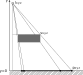
\includegraphics[width=0.5\textwidth]{./graf/projection_shadow.pdf}
	\caption{Vertices of a shadow caster projected onto \(y=0\) plane create a planar shadow. Dashed lines visualize the similar triangles.}
	\label{fig:projection_shadow}
\end{figure}

Using this geometric understanding and similar triangles, marked in Fig. \ref{fig:projection_shadow} in dashed lines, the following equations and a projection matrix can be derived. Assuming \(l\) to be the position of a light source, \(v\) to be the position of a vertex of the shadow caster and \(p\) the position of the projected shadow vertex, a projection onto the \(y=0\) plane is described by:

\begin{align}
	\frac{p_x - l_x}{v_x - l_x} = \frac{l_y}{l_y - v_y} \Longleftrightarrow p_x = \frac{l_yv_x - l_xv_y}{l_y - v_y}
\end{align}

The \(z\) component is derived in analogous way:

\begin{align}
	\frac{p_z - l_z}{v_z - l_z} = \frac{l_y}{l_y - v_y} \Longleftrightarrow p_z = \frac{l_yv_z - l_zv_y}{l_y - v_y}
\end{align}

The \(y\) component will be \(y=0\) since the projection happens onto the \(xz\) plane. From that the projection matrix can be constructed:

\begin{align}
	\mathbf{M} = 
	\begin{pmatrix}
		l_y & -l_x & 0 & 0\\
		0 & 0 & 0 & 0\\
		0 & -l_z & l_y & 0\\
		0 & -1 & 0 & l_y
	\end{pmatrix}
\end{align}

The \(l_y - v_y\) factor in the denominator is obtained by utilizing the property of homogenous coordinates, where all components of a vector \(\mathbf{v} = \begin{bmatrix}x & y & z & w\end{bmatrix}^T\) get divided by the \(w\) component, which gives \(\mathbf{v} = \begin{bmatrix}x/w & y/w & z/w & 1\end{bmatrix}^T\).

This matrix can be generalized to project points onto any plane, but this was not implemented.

In the implementation the matrix is created in the vertex shader based on the position of the light source. The vertices of the caster, after being transformed into world space, are multiplied by it, projecting them onto the \(y=0\) plane. Then they are transformed with the view and perspective projection matrices as usual. The resulting mesh is rendered in black, with a pixel shader that just returns the black color. Special care should be taken when rendering the shadow mesh, since it perfectly overlaps the ground plane at \(y=0\). To avoid z-fighting, which is shown in Fig \ref{fig:projection_shadow_beyond}, this mesh needs to be rendered after the receiver and before the caster, with z depth testing turned off in the rendering pipeline, or, as is the case in the implementation, a negative depth offset needs to be added to the mesh to bring it above the ground plane.

\begin{figure}[h]
    \centering
    \begin{subfigure}[t]{0.45\textwidth}
		\centering
        \includegraphics[width=\textwidth]{./graf/projection_shadow_beyond.png}
        \caption{The projected shadow mesh lies beyond the ground plane.}
        \label{fig:projection_shadow_beyond}
    \end{subfigure}
	\hfill
    \begin{subfigure}[t]{0.45\textwidth}
		\centering
        \includegraphics[width=\textwidth]{./graf/projection_shadow_fighting.png}
        \caption{Severe z-fighting caused by the fact that both the ground plane mesh and shadow mesh lie in the exact same plane.}
        \label{fig:projection_shadow_fighting}
    \end{subfigure}

    \caption{Some of the issues that can arise when using projection shadows.}
    \label{fig:projection_shadow_issues}
\end{figure}

\begin{figure}[h]
	\centering
	\includegraphics[width=0.3\textwidth]{./graf/projection_anti_shadow.pdf}
	\caption{The shadow caster projected through a light source, creating an anti-shadow.}
	\label{fig:projection_anti_shadow}
\end{figure}

Multiple issues arise with this technique. The receiver must be a flat plane, objects cannot shadow themselves, casters and receivers need separate treatment. Additionally, care needs to be taken to only render the shadow meshes on top of the geometry of a receiver. Since the shadow is a separate mesh, it could be cast beyond the actual surface of the receiver, creating an impossible shadow in the air. This is illustrated in Fig \ref{fig:projection_shadow_fighting} There is another possibility here for an impossible shadow. If the light source is between the caster and receiver, an anti-shadow will be cast as shown in Fig \ref{fig:projection_anti_shadow}. This creates another special case that needs to be checked for by the application. Soft shadows are also difficult and costly to achieve, created by projecting the caster geometry multiple times using different discrete locations sampled over the area of the light source. The shadow meshes can then be blended, producing a darker color where more shadows are present. This gives very accurate results with a high number of samples, but is not a viable option for real-time rendering. All these problems make this technique virtually unused in modern rendering engines.

% TODO: add some notes on performance.

\subsection{Implementation of basic shadow mapping}
\label{section:basic_mapping_impl}
As mentioned in chapter \ref{section:basic_mapping}, shadow mapping for a single light source is performed using two render passes. The first one generates the shadow map itself, the second and final pass renders the scene with shadows determined using the shadow map. The shadow map is a z-buffer, which means that, for each texel, it stores the values of the z coordinate of the scene surface point being rendered. These coordinates are stored after transforming the vertices of the scene into the NDC space, or normalized device coordinate space, of a given light source. This transformation is achieved in the vertex shader, by using the regular world, view, projection (WVP) transformation matrices, with the distinction that the view and projection matrices are not of the scene observer but of the light source. In truth, multiplying the vertex positions by the WVP matrix will result in clip space homogenous coordinates, which then will be transformed automatically by the pipeline into NDC during the perspective division, when the homogenous coordinates are divided by their \(w\) component. The stored depth values will then be in the \(0-1\) range, usually \(0\) being at the near clipping plane and \(1\) at the far clipping plane. This z-buffer can then be used as a texture shader resource in a pixel shader to render the final scene. To read the depth values from the shadow map, the NDC coordinates of each surface point need to be calculated again. The \(x\) any \(y\) components will then be used to access a texel in the shadow map, the \(z\) component will be compared with the contents of the shadow map. Do note that the actual Euclidean distance between the shaded point and the light source is not used, as these values would be in different coordinate spaces. When the shadow map value is accessed, it is compared with the \(z\) value of the point that is currently being shaded. If the shadow map value is greater, then the point being shaded is farther away from the light source than some other surface seen at this point from the point of view of the light. This means that it is not illuminated and is in shadow. Otherwise, the point is lit by the light source. The process is illustrated in Fig. \ref{fig:shadow_map_basic}. Fig. \ref{fig:shadow_map_screens} shows a rendered view of a scene with shadow mapping and the shadow map itself.


\begin{figure}[hp]
	\centering
	\includegraphics[width=0.5\textwidth]{./graf/shadow_mapping_basic.pdf}
	\caption{The light source \(l\) has stored the depth value \(z_l\) in its shadow map. When rendering the scene from the viewpoint of the observer \(v\), the stored depth is compared to the depth \(z_v\). This value will be larger than the one in the shadow map, so the point will be in shadow.}
	\label{fig:shadow_map_basic}
\end{figure}

\begin{figure}[hbp]
    \centering
    \begin{subfigure}{0.45\textwidth}
		\centering
        \includegraphics[width=\textwidth]{./graf/shadow_mapping_basic_sponza.png}
        \caption{A scene rendered with the use of shadow mapping.}
        \label{fig:shadow_map_screens_scene}
    \end{subfigure}
	\hfill
    \begin{subfigure}{0.45\textwidth}
		\centering
        \includegraphics[width=\textwidth]{./graf/shadow_mapping_basic_depth_map.png}
        \caption{Section of the shadow map rendered for this scene.}
        \label{fig:shadow_map_screens_depth}
    \end{subfigure}

    \caption{An example scene rendered with a shadow map, which is shown in black and white.}
    \label{fig:shadow_map_screens}
\end{figure}

To implement this technique a resource is needed that will be used both as an additional depth buffer and a texture. This can be easily achieved in an application programming interface (API) like DirectX 12 by creating one resource and two resource views, one being a Depth Stencil View (DSV) and another a Shader resource view (SRV). Once the rendering of the shadow map is finished using the DSV, the resource can be transitioned in preparation to be used as an SRV during rendering the main view using a resource barrier. Caution needs to be taken to transition the resource back to a DSV-compatible state before rendering the shadow map of the next frame. In this case, a resource barrier will also ensure that all write operations have finished before continuing with rendering, meaning that the rendering of the shadow map will be complete before it is used in the final pass. The shaders responsible for rendering the main scene view will evidently need access to the texture resource containing the shadow map, but also it will need to access the view and projection matrices of the light view pass. This is to calculate the corresponding NDC coordinates of the point being shaded in the shadow map. It is optimal to calculate light clip space coordinates in the vertex shader and let the pipeline interpolate them across the triangle for each fragment. Since the perspective division will not happen automatically here, it is needed to divide the coordinates by the \(w\) component in the pixel shader to obtain correct NDC values. Since the shadow map is sampled as a texture, the \(xy\) coordinates with range \([-1:1]\) need to be converted into \(uv\) texture coordinates with range \([0:1]\). Additionally, the \(y\) component needs to be flipped to address the texture correctly. This can be performed as a simple transformation in the pixel shader as \(\begin{bmatrix}x & y\end{bmatrix}^T /  \begin{bmatrix}2 & -2\end{bmatrix}^T + \begin{bmatrix}0.5 & 0.5\end{bmatrix}^T\) or incorporated into the MVP matrix of the light view. This can be achieved by multiplying the MVP matrix for the light source by the offset matrix as shown in equation \ref{eq:offset_matrix_shadow_mapping}.

\begin{align}
	\label{eq:offset_matrix_shadow_mapping}
	\mathbf{L_{offset}} = 
	\begin{pmatrix}
		0.5 & 0 & 0 & 0.5\\
		0 & -0.5 & 0 & 0.5\\
		0 & 0 & 1 & 0\\
		0 & 0 & 0 & 1
	\end{pmatrix}
	\cdot \mathbf{MVP}
\end{align}

When sampling the shadow map as a texture, it is important to do so with a sampler that does not perform any filtering on the texture. Typically, texture filtering helps avoid different kinds of aliasing. Regular color textures however can be filtered and interpolated as they only store color data. The shadow map, which stores depth values, cannot be filtered in the same way as the produced values would be senseless in this process. They would create non-existing apparent surfaces especially noticeable between sharp depth changes, for example between a close object and the far clipping plane.

This observation brings forth one of the issues with shadow mapping: they cannot be filtered to avoid aliasing. One could also attempt to blur a shadow map to achieve soft shadows, but this is not a viable option for the same reason. Because of this basic shadow mapping can only be used to create hard shadows that suffer from aliasing issues, creating shadows that can appear blocky when up close, as in Fig. \ref{fig:shadow_mapping_blocky}. Aliasing can be mitigated by rendering the shadow map into a higher resolution target, but only to a degree. Special techniques allowing for smoothing and filtering shadows generated with shadow mapping will be presented in the following sections.

\begin{figure}
    \centering
	\includegraphics[width=0.7\textwidth]{./graf/shadow_mapping_blocky.png}
	\caption{Aliased shadow appearance due to no filtering and low resolution of the shadow map.}
	\label{fig:shadow_mapping_blocky}
\end{figure}

When rendering the shadow map an appropriate projection matrix has to be constructed. For a far away directional light, such as a sun light, an orthographic projection should be used. When rendering a spotlight a perspective projection can be used. Point lights can also use a single shadow map with a perspective projection matrix, but only in situations when the light source is positioned outside the scene, or at least is not surrounded by shadow casters. In the opposite case, the most common technique is to use cubemaps and improved derivative techniques as described by Liang Wan \cite{bib:article:wan_cubemaps}. A cubemap consists of six shadow map renders, each covering a face of a cube constructed around the light source. This way an omnidirectional shadow map is created.

When creating a projection matrix as well as the view matrix for a shadow map, care has to be taken to capture all relevant shadow casters. This is especially true for large scale scenes and directional lights, as rendering the entirety of a scene into the shadow map would most of the time be unnecessary and suboptimal. Most of the rendered map would not be used in a given frame, and the distribution of shadow map resolution would be poor. It would be enough for the light view to tightly encompass the view frustum of the observer to obtain correct results. This is called fitting and will be presented in the following sections. This idea can be taken further as shown by Ji\v{r}\'{\i} Bittner \cite{bib:proc:bittner_caster_culling} to allow for an approximate FPS gain of 1.5 times. Their method uses a custom advanced algorithm to cull shadow casters and render only those that contribute to the current main viewpoint.

Another issue of shadow maps is self-shadowing, or surface acne. This is also a result of aliasing, since the continuous scene geometry and its depth data is sampled in a discrete manner into an image when rendering the shadow map. If the shadow map texel does not correlate one-to-one with the final view samples, which happens very often and is highly likely, the shadow map samples will cover a non-zero area on the geometry surface in the final view of the scene, which is illustrated in Fig. \ref{fig:shadow_mapping_acne_explanation}.
\begin{figure}[hp]
	\centering
	\begin{subfigure}{0.7\textwidth}
        \includegraphics[width=\textwidth]{./graf/shadow_mapping_acne.pdf}
        \caption{Depth samples being compared with depth values over an area of the actual mesh lead to aliasing and shadow acne.}
        \label{fig:shadow_mapping_acne_explanation_3d}
    \end{subfigure}
	\begin{subfigure}{0.7\textwidth}
        \includegraphics[width=\textwidth]{./graf/shadow_mapping_acne_side.pdf}
        \caption{The aliasing issue present in shadow maps illustrated in two dimensions from the side.}
        \label{fig:shadow_mapping_acne_explanation_side}
    \end{subfigure}

    \caption{The cause of shadow acne. Light source \(l\) renders the shadow map onto its projection plane \(p\), having some finite resolution. The sampled depth value \(z\) is stored in a texel. This creates a virtual surface orthogonal to the light direction on top of the actual geometry surface \(s\). When rendering the scene, depth values in the area \(a_1\) will have a lower depth value stored in the shadow map texel than their actual depth, causing them to be in light. Samples in the \(a_2\) area will have greater depth, causing them to be evaluated as being in shadow.}
    \label{fig:shadow_mapping_acne_explanation}
\end{figure}
This can cause the surface to erroneously shadow itself, as shown in Fig. \ref{fig:shadow_mapping_acne}. This issue gets more pronounced the higher the angle between the light source view ray and the surface normal. It can be resolved by adding a depth bias when rendering the shadow map, which will ensure the samples are below the actual surface. In modern rendering APIs the depth bias can be configured for a pipeline and applied automatically when rendering. Especially useful is the combination of a constant depth bias and a slope-scaled depth bias. The second bias helps eliminate the problem when surfaces appear more edge-on in the light view by scaling the depth bias with the angle between the light direction and surface. Too high depth bias can cause peter-panning, a situation shown in Fig. \ref{fig:shadow_mapping_panning} where a shadow caster gets detached from its shadow. Because of this, depth bias values often need to be hand-tuned on a per-scene basis. Other approaches have also been proposed, such as using only the back faces of objects to render the shadow map \cite{bib:rep:wang_second_depth_mapping} or utilizing depth peeling to store average depths between the back and front faces of an object \cite{bib:book:woo_midpoint_depth_map}, but they both still require some bias to avoid shadow-acne in areas such as silhouette edges or concavities.

\begin{figure}[h]
    \centering
    \begin{subfigure}{0.45\textwidth}
		\centering
        \includegraphics[width=\textwidth]{./graf/shadow_mapping_acne.png}
        \caption{Shadow acne due to using not enough bias.}
        \label{fig:shadow_mapping_acne}
    \end{subfigure}
	\hfill
    \begin{subfigure}{0.45\textwidth}
		\centering
        \includegraphics[width=\textwidth]{./graf/shadow_mapping_panning.png}
        \caption{The cube is disconnected from its shadow due to too much depth bias.}
        \label{fig:shadow_mapping_panning}
    \end{subfigure}

    \caption{Some of the issues that can arise when using projection shadows.}
    \label{fig:shadow_mapping_issues}
\end{figure}

The z-buffer of a rendered image can be actually non-linear in its \([0-1]\) range. Perspective projection matrices are sometimes built in such a way that the precision closer to \(1\) is lower than closer to \(0\). This is purposefully done to gain more precision closer to the viewer, where it is more needed when performing hidden-surface removal than far away, where objects will become very small due to perspective foreshortening. This can be an issue with shadow mapping, since objects close to the light source are not necessarily close to the viewer. In fact the opposite can often be true. As shown by Stefan Brabec \cite{bib:article:brabec_linear_depth}, the z-buffer for the use in shadow mapping can be linearized using a linear transformation dependent on the projection matrix used. The following perspective projection matrix present in the DX Math library can be linearized with equation \ref{eq:projection_linearization}.

\begin{gather}
	\label{eq:projection_perspective}
	\begin{pmatrix}
		W & 0 & 0 & 0\\
		0 & H & 0 & 0\\
		0 & 0 & \frac{f}{f-n} & \frac{-fn}{f-n}\\
		0 & 0 & 1 & 0
	\end{pmatrix}
    \begin{pmatrix}
		x\\
		y\\
		z\\
		w
	\end{pmatrix} =
    \begin{pmatrix}
		Wx\\
		Hy\\
		\frac{zf}{f-n} - \frac{wfn}{f-n}\\
		z
	\end{pmatrix} \Rightarrow 
    \begin{pmatrix}
		Wx\\
		Hy\\
		\frac{zf}{f-n} - \frac{fn}{f-n}\\
		z
	\end{pmatrix}
    \quad \text{for} \quad w = 1\\[10pt]
    \begin{pmatrix}
		Wx\\
		Hy\\
		\frac{zf}{f-n} - \frac{fn}{f-n}\\
		z
	\end{pmatrix} / z =
    \begin{pmatrix}
		\frac{Wx}{z}\\
		\frac{Hy}{z}\\
		\frac{f}{f-n} - \frac{fn}{z(f-n)}\\
		1
	\end{pmatrix}
\end{gather}

After the perspective division the final form of the z-value equation is obtained. Below, in Fig. \ref{plot:perspective_z}, the z-values are plotted for exemplary near and far clipping planes equal \(n=2\), \(f=15\).

\begin{figure}[h]
    \centering
    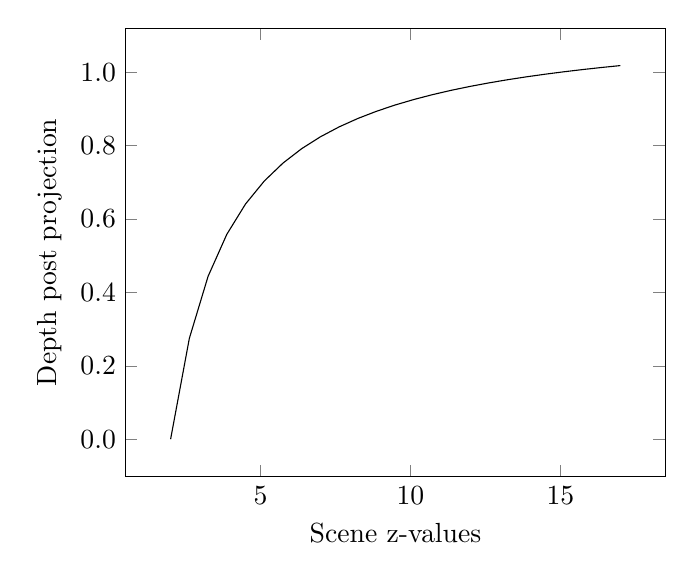
\begin{tikzpicture}
    \begin{axis}[
        xlabel=Scene z-values,ylabel=Depth post projection,
        y tick label style={
            /pgf/number format/.cd,
                fixed,   % po zakomentowaniu os rzednych jest indeksowana wykladniczo
                fixed zerofill, % 1.0 zamiast 1
                precision=1,
            /tikz/.cd
        },
        x tick label style={
            /pgf/number format/.cd,
                fixed,
                fixed,
                precision=2,
            /tikz/.cd
        }
    ]
    \addplot [domain=2.0:17.0] {(15/13)-(30/(13*x))};
    \end{axis} 
    \end{tikzpicture}
    \caption{The z-values after a perspective projection become non-linear.}
    \label{plot:perspective_z}
\end{figure}

The values can be linearized back again simply by multiplying the clip-space z-value by \(\frac{z}{f}\), which gives the following equation.

\begin{align}
	\label{eq:projection_linearization}
	\left(\frac{f}{f-n} - \frac{fn}{z(f-n)}\right) * \frac{z}{f} = \frac{z-n}{f-n}
\end{align}

In the application z-buffer linearization was not implemented, as after investigation it turned out that an orthographic projection, which is used for the directional light, does not introduce nonlinearity to the z-buffer range. This can be seen by inspecting how the matrix will affect the \(w\) component. The orthographic projection matrix as implemented in the DX Math library is presented below.

\begin{align}
	\label{eq:projection_ortho}
	\mathbf{M_{o}} = 
	\begin{pmatrix}
		W & 0 & 0 & 0\\
		0 & H & 0 & 0\\
		0 & 0 & \frac{1}{f-n} & \frac{-n}{f-n}\\
		0 & 0 & 0 & 1
	\end{pmatrix}
\end{align}

This matrix does not modify the \(w\) component and the \(z\) values will remain linear. In fact the formula for depth values after using this matrix is exactly the same as the perspective one after linearization.

\subsection{Fitting shadow maps}
An attempt to implement LiSPSM was made, but was not successful due to poor coverage of the implementation details both in the original paper and on the internet.

Only a part of the algorithm was implemented, basically providing simplified fitting of the shadow map view. The shadow map camera has certain extents set up by hand for each scene, such that the whole scene fits within view. Since the entire scene is not necessarily viewed at once by the observer, only the part that is within the observer view frustum can be rendered to the shadow map. Therefore, the shadow map post-projection space can be adjusted to include the area viewed by the observer.

This can be achieved by building a fitting transformation matrix \(\mathbf{F}\) that includes translation and scaling, that is applied after the light view and projection matrices, resulting in \(\mathbf{F}\mathbf{P}_L\mathbf{V}_L\). To obtain \(\mathbf{F}\), first the observer view frustum extents need to be found in world space, which can be obtained by applying the inverse of observer view and projection matrices to an NDC cuboid. This can be a cube with ranges \([-1:1]\) in \(x\), \(y\), \(z\) in APIs like OpenGL, or a cuboid with ranges \([-1:1]\) in \(x\) and \(y\), and \([0:1]\) in \(z\) in DirectX. Once the vertices of this cuboid are moved into world space, they can be multiplied by the view and projection matrices of the light source, \(\mathbf{P}_L\mathbf{V}_L\), and their components divided by \(w\) to bring them into the post-projection space of the light source. Once there, a bounding box can be found enclosing these points. To not move the contents of the shadow map beyond the original extent specified for the light source, the components of the vertices of this bounding box can be clamped to the NDC range. The whole process is shown in Fig. \ref{fig:shadow_map_fitting}.
\begin{figure}
    \centering
	\includegraphics[width=0.4\textwidth]{./graf/shadow_map_focusing.pdf}
	\caption{The steps involved in fitting the shadow map. The NDC cuboid in a) is in observer post-projection space, or clip space. It is moved to the state presented in b) using inverse matrices, resulting in a world space representation of the viewing frustum. It is them transformed into c), the light view clipping space. Finally, a clamped bounding box is found, shown in d).}
	\label{fig:shadow_map_fitting}
\end{figure}
Finally, the minimum and maximum \(x\) and \(y\) values of these bounding vertices can be found and used in the following fitting matrix.
\begin{align}
	\mathbf{F} &= 
	\begin{pmatrix}
		s_x & 0 & 0 & o_x\\
		0 & s_y & 0 & o_y\\
		0 & 0 & 1 & 0\\
		0 & 0 & 0 & 1
	\end{pmatrix}, \text{where}\\[10pt]
	s_x &= \frac{2}{x_{max} - x_{min}} \quad\text{and}\quad o_x = \frac{-s_x(x_{max} + x_{min})}{2}
\end{align}
The calculation of \(s_y\) and \(o_y\) is analogous.

As was implemented, the fitting focuses on an approximate convex body of \(\mathbf{L}\cap \mathbf{V}\), where \(\mathbf{L}\) stands for the light view frustum and \(\mathbf{V}\) for the viewer frustum. The shadow map is then fitted only in the clip space \(x\) and \(y\) dimensions, ignoring depth \(z\). A more robust solution would be to find the convex hull of \(\mathbf{L}\cap \mathbf{V}\cap \mathbf{S}\), with \(\mathbf{S}\) meaning the scene bounding box. Then the shadow map would only focus on areas within the viewer frustum where there exists geometry to render. The near plane of the light frustum can then be set to the upper scene extent and the far plane to the farthest viewer frustum point. The shadow map would then require no hand adjustments to its frustum and would adapt to different scenes and viewer orientations.

\subsection{Some other shadow maps}

% \begin{itemize}
% \item solution to the problem proposed by the author of the thesis
% \item theoretical analysis of proposed solutions
% \item rationale of applied methods, algorithms, and tools
% \end{itemize}

% Here I should describe my reasoning for the testing, reasoning for
% selecting the techniques that I do select, my program for testing.

% \section{[Section title]}

% \section{[Subsection title]}

% Each figure in the document should be referred to at least once (fig. \ref{fig:2}).

% \begin{figure}
% \centering
% \begin{tikzpicture}
% \begin{axis}[
%     y tick label style={
%         /pgf/number format/.cd,
%             fixed,   % po zakomentowaniu os rzednych jest indeksowana wykladniczo
%             fixed zerofill, % 1.0 zamiast 1
%             precision=1,
%         /tikz/.cd
%     },
%     x tick label style={
%         /pgf/number format/.cd,
%             fixed,
%             fixed zerofill,
%             precision=2,
%         /tikz/.cd
%     }
% ]
% \addplot [domain=0.0:0.1] {rnd};
% \end{axis} 
% \end{tikzpicture}
% \caption{Figure caption.} % Figure caption is BELOW the figure!
% \label{fig:2}
% \end{figure}


%%%%%%%%%%%%%%%%%%%%%
% FIGURE FROM FILE
%
%\begin{figure}
%\centering
%\includegraphics[width=0.5\textwidth]{./graf/politechnika_sl_logo_bw_pion_en.pdf}
%\caption{Caption of a figure is always below the figure.}
%\label{fig:label}
%\end{figure}
%Fig. \ref{fig:label} presents …
%%%%%%%%%%%%%%%%%%%%%
%
%%%%%%%%%%%%%%%%%%%%
%% SUBFIGURES
%
%\begin{figure}
%\centering
%\begin{subfigure}{0.4\textwidth}
%    \includegraphics[width=\textwidth]{./graf/politechnika_sl_logo_bw_pion_en.pdf}
%    \caption{Upper left figure.}
%    \label{fig:upper-left}
%\end{subfigure}
%\hfill
%\begin{subfigure}{0.4\textwidth}
%    \includegraphics[width=\textwidth]{./graf/politechnika_sl_logo_bw_pion_en.pdf}
%    \caption{Upper right figure.}
%    \label{fig:upper-right}
%\end{subfigure}
%
%\begin{subfigure}{0.4\textwidth}
%    \includegraphics[width=\textwidth]{./graf/politechnika_sl_logo_bw_pion_en.pdf}
%    \caption{Lower left figure.}
%    \label{fig:lower-left}
%\end{subfigure}
%\hfill
%\begin{subfigure}{0.4\textwidth}
%    \includegraphics[width=\textwidth]{./graf/politechnika_sl_logo_bw_pion_en.pdf}
%    \caption{Lower right figure.}
%    \label{fig:lower-right}
%\end{subfigure}
%        
%\caption{Common caption for all subfigures.}
%\label{fig:subfigures}
%\end{figure}
%Fig. \ref{fig:subfigures} presents very important information, eg. Fig. \ref{fig:upper-right} is an upper right subfigure.
%%%%%%%%%%%%%%%%%%%%%


% Each table in the document should be referred to at least once (Tab. \ref{tab:results}).

% \begin{table}
% \centering
% \caption{A caption of a table is ABOVE it.}
% \label{tab:results}
% \begin{tabular}{rrrrrrrr}
% \toprule
% 	         &                                     \multicolumn{7}{c}{method}                                      \\
% 	         \cmidrule{2-8}
% 	         &         &         &        \multicolumn{3}{c}{alg. 3}        & \multicolumn{2}{c}{alg. 4, $\gamma = 2$} \\
% 	         \cmidrule(r){4-6}\cmidrule(r){7-8}
% 	$\zeta$ &     alg. 1 &   alg. 2 & $\alpha= 1.5$ & $\alpha= 2$ & $\alpha= 3$ &   $\beta = 0.1$  &   $\beta = -0.1$ \\
% \midrule
% 	       0 &  8.3250 & 1.45305 &       7.5791 &    14.8517 &    20.0028 & 1.16396 &                       1.1365 \\
% 	       5 &  0.6111 & 2.27126 &       6.9952 &    13.8560 &    18.6064 & 1.18659 &                       1.1630 \\
% 	      10 & 11.6126 & 2.69218 &       6.2520 &    12.5202 &    16.8278 & 1.23180 &                       1.2045 \\
% 	      15 &  0.5665 & 2.95046 &       5.7753 &    11.4588 &    15.4837 & 1.25131 &                       1.2614 \\
% 	      20 & 15.8728 & 3.07225 &       5.3071 &    10.3935 &    13.8738 & 1.25307 &                       1.2217 \\
% 	      25 &  0.9791 & 3.19034 &       5.4575 &     9.9533 &    13.0721 & 1.27104 &                       1.2640 \\
% 	      30 &  2.0228 & 3.27474 &       5.7461 &     9.7164 &    12.2637 & 1.33404 &                       1.3209 \\
% 	      35 & 13.4210 & 3.36086 &       6.6735 &    10.0442 &    12.0270 & 1.35385 &                       1.3059 \\
% 	      40 & 13.2226 & 3.36420 &       7.7248 &    10.4495 &    12.0379 & 1.34919 &                       1.2768 \\
% 	      45 & 12.8445 & 3.47436 &       8.5539 &    10.8552 &    12.2773 & 1.42303 &                       1.4362 \\
% 	      50 & 12.9245 & 3.58228 &       9.2702 &    11.2183 &    12.3990 & 1.40922 &                       1.3724 \\
% \bottomrule
% \end{tabular}
% \end{table}  


% \begin{figure}
% \centering
% \includegraphics[width=0.5\textwidth]{./graf/test_image.jpg}
% \caption{Caption of a figure is always below the figure akakak.}
% \label{fig:duped_image4}
% \end{figure}

% some citation of the above \ref{fig:duped_image4}


\chapter{Experiments}
\label{section:chapter_4}
% This chapter presents the experiments. It is a crucial part of the thesis and has to dominate in the thesis. 
% The experiments and their analysis should be done in the way commonly accepted in the scientific community (eg. benchmark datasets, cross validation of elaborated results, reproducibility and replicability of tests etc).

\section{Methodology}
% \begin{itemize}
% \item description of methodology of experiments
% \item description of experimental framework (description of user interface of research applications – move to an appendix)
% \end{itemize}
One of the objectives of the thesis was to compare multiple shadow rendering methods both in a qualitative and quantitative ways. To achieve this a test renderer application was created, which implements the rendering techniques and allows a user to observe their results as well as profile the performance the program.

The tests were performed in a semi-controlled environment. Care was taken to avoid other processes interrupting and affecting the test results, but their impact could not be entirely eliminated in. Results of repeated tests at different moments in time or on different machines with the same hardware will differ, but that difference should not be large enough to impact the overall comparison results. 
% TODO: if you use two machines, mention it here.
The machine used for performing measurements had the following specification:
\begin{itemize}
    \item OS: Windows 10, 22H2
    \item CPU: AMD Ryzen 5 1600
    \item GPU: Nvidia GTX 1080, 8 GB VRAM
    \item RAM: 16 GB
\end{itemize}

\subsection{Created test application}
The test application allows the user to choose a rendering mode and observe the results in real time. It also allows to change the viewpoint and observe how the shadows behave in motion. Most rendering modes implement different shadow rendering techniques and some include debug views like wireframe mode or mesh colored by normals. The application is also instrumented with profiling commands which make it possible to connect to an external profiler and collect data in real time, as well as save and load existing profiling data.

As mentioned in section \ref{chapter:3_test_app}, the Tracy profiler open source library and tool was used to gather and visualize profiling data. For additional profiling and debugging RenderDoc, PIX and Nsight Graphics were used.

\section{Data sets}
The data sets consist of multiple scenes used for testing. Three scenes, Crytek Sponza, Power Plant and Chinese Dragon are from the Computer Graphics Archive \cite{bib:internet:test_scenes}. The Crytek Sponza scene contains 262267 triangles and 184330 vertices. The Power Plant scene contains 12759246 triangles and 10614919 vertices. The Chinese Dragon contains 871306 triangles and 438929 vertices. They were chosen because they are standard test scenes in the computer graphics community, which are freely available on the internet. They also contain highly varying amounts of vertices, with the Power Plant scene having almost sixty times more vertices than Cytek Sponza, which allows to test the influence of geometric complexity on the performance of the algorithms. The Chinese Dragon scene is much more contained and showcases small-scale shadows and self-shadowing. Additionally, a simple scene containing a unit cube positioned on a ground plane was created in Blender. This scene contains only twenty-eight vertices. Its simplicity allows to easily spot differences in the appearance of shadows in the render and highlights issues such as peter-panning.

\section{Results}
% \begin{itemize}
% \item presentation of results, analysis and wide discussion of elaborated results, conclusions
% \end{itemize}

The results of testing each implemented shadow rendering method are presented in the following sections. Each set of results is complemented by a description and discussion.

\subsection{Planar shadow mapping}
Should I even test this?
% TODO.

\subsection{Basic shadow maps}
The basic implementation of shadow mapping from section \ref{section:basic_mapping_impl} was tested with all four scenes at different shadow map and output resolutions. The results are shown in Fig. \ref{fig:plot:basic_results}.
\begin{figure}[h]
\centering
\begin{subfigure}[t]{0.48\textwidth}
    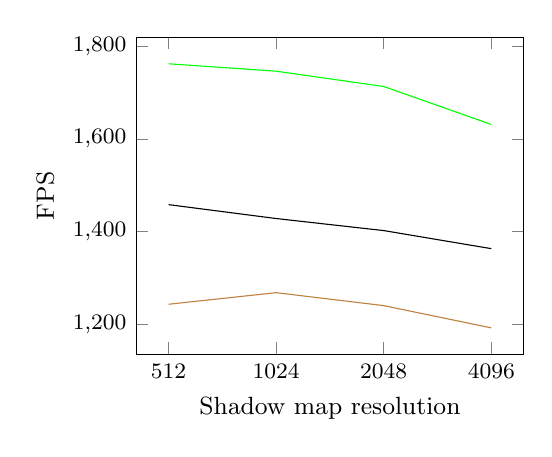
\begin{tikzpicture}
        \begin{semilogxaxis}[
            small,
            xlabel={Shadow map resolution},
            ylabel={FPS},
            xtick={512,1024,2048,4096},
            xticklabels={512,1024,2048,4096},
            % legend style={
            %     overlay,
            %     at={(1.25,0.5)},
            %     anchor=center},
            y tick label style={
                /pgf/number format/.cd,
                    fixed,   % po zakomentowaniu os rzednych jest indeksowana wykladniczo
                    fixed, % 1.0 zamiast 1
                    precision=1,
                /tikz/.cd
            },
            x tick label style={
                /pgf/number format/.cd,
                    fixed,
                    fixed,
                    precision=2,
                /tikz/.cd
            }
            ]
            \addplot [color=green]
            coordinates {
                (512,1762)(1024,1746)(2048,1713)(4096,1631)}; %\addlegendentry{720p}
            \addplot [color=black]
            coordinates {
                (512,1458)(1024,1428)(2048,1402)(4096,1363)}; %\addlegendentry{1080p}
            \addplot [color=brown]
            coordinates {
                (512,1243)(1024,1268)(2048,1240)(4096,1192)}; %\addlegendentry{2k}
        \end{semilogxaxis} 
    \end{tikzpicture}
    \caption{Results for Chinese Dragon scene.}
    \label{fig:plot:basic_dragon}
\end{subfigure}
\hfill
\begin{subfigure}[t]{0.48\textwidth}
    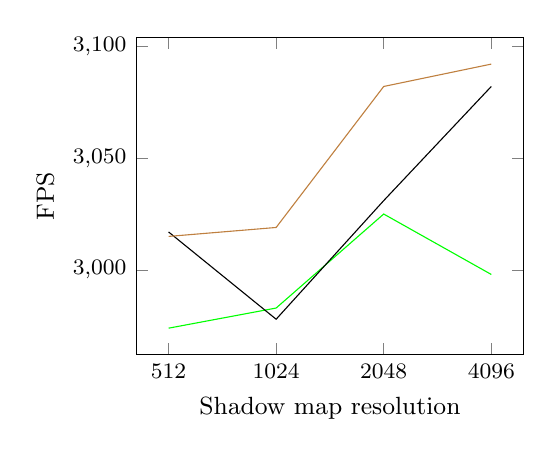
\begin{tikzpicture}
        \begin{semilogxaxis}[
            small,
            xlabel={Shadow map resolution},
            ylabel={FPS},
            xtick={512,1024,2048,4096},
            xticklabels={512,1024,2048,4096},
            % legend style={
            %     overlay,
            %     at={(1.25,0.5)},
            %     anchor=center},
            y tick label style={
                /pgf/number format/.cd,
                    fixed,   % po zakomentowaniu os rzednych jest indeksowana wykladniczo
                    fixed, % 1.0 zamiast 1
                    precision=1,
                /tikz/.cd
            },
            x tick label style={
                /pgf/number format/.cd,
                    fixed,
                    fixed,
                    precision=2,
                /tikz/.cd
            }
            ]
            \addplot [color=green]
            coordinates {
                (512,2974)(1024,2983)(2048,3025)(4096,2998)}; %\addlegendentry{720p}
            \addplot [color=black]
            coordinates {
                (512,3017)(1024,2978)(2048,3031)(4096,3082)}; %\addlegendentry{1080p}
            \addplot [color=brown]
            coordinates {
                (512,3015)(1024,3019)(2048,3082)(4096,3092)}; %\addlegendentry{2k}
        \end{semilogxaxis} 
    \end{tikzpicture}
    \caption{Results for the Cube scene.}
    \label{fig:plot:basic_cube}
\end{subfigure}

\vspace{20pt}
\begin{subfigure}[t]{0.48\textwidth}
    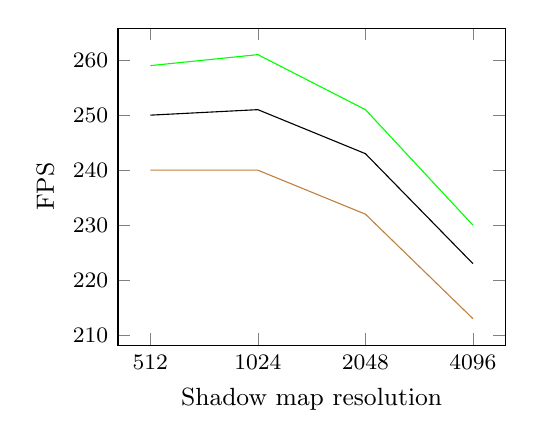
\begin{tikzpicture}
        \begin{semilogxaxis}[
            small,
            xlabel={Shadow map resolution},
            ylabel={FPS},
            xtick={512,1024,2048,4096},
            xticklabels={512,1024,2048,4096},
            % legend style={
            %     overlay,
            %     at={(1.25,0.5)},
            %     anchor=center},
            y tick label style={
                /pgf/number format/.cd,
                    fixed,   % po zakomentowaniu os rzednych jest indeksowana wykladniczo
                    fixed, % 1.0 zamiast 1
                    precision=1,
                /tikz/.cd
            },
            x tick label style={
                /pgf/number format/.cd,
                    fixed,
                    fixed,
                    precision=2,
                /tikz/.cd
            }
            ]
            \addplot [color=green]
            coordinates {
                (512,259)(1024,261)(2048,251)(4096,230)}; %\addlegendentry{720p}
            \addplot [color=black]
            coordinates {
                (512,250)(1024,251)(2048,243)(4096,223)}; %\addlegendentry{1080p}
            \addplot [color=brown]
            coordinates {
                (512,240)(1024,240)(2048,232)(4096,213)}; %\addlegendentry{2k}
        \end{semilogxaxis} 
    \end{tikzpicture}
    \caption{Results for the Power Plant scene.}
    \label{fig:plot:basic_power}
\end{subfigure}
\hfill
\begin{subfigure}[t]{0.48\textwidth}
    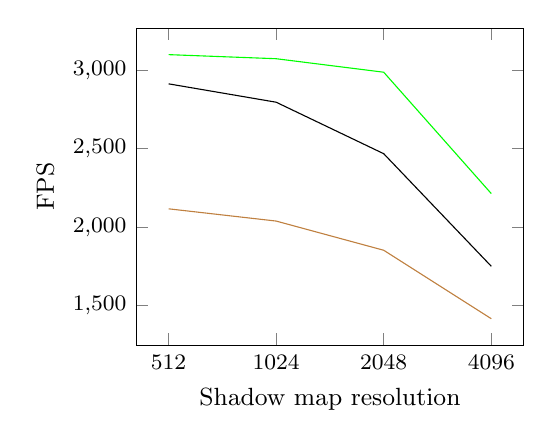
\begin{tikzpicture}
        \begin{semilogxaxis}[
            small,
            xlabel={Shadow map resolution},
            ylabel={FPS},
            xtick={512,1024,2048,4096},
            xticklabels={512,1024,2048,4096},
            % legend style={
            %     overlay,
            %     at={(1.25,0.5)},
            %     anchor=center},
            y tick label style={
                /pgf/number format/.cd,
                    fixed,   % po zakomentowaniu os rzednych jest indeksowana wykladniczo
                    fixed, % 1.0 zamiast 1
                    precision=1,
                /tikz/.cd
            },
            x tick label style={
                /pgf/number format/.cd,
                    fixed,
                    fixed,
                    precision=2,
                /tikz/.cd
            }
            ]
            \addplot [color=green]
            coordinates {
                (512,3098)(1024,3072)(2048,2986)(4096,2213)}; %\addlegendentry{720p}
            \addplot [color=black]
            coordinates {
                (512,2912)(1024,2795)(2048,2467)(4096,1750)}; %\addlegendentry{1080p}
            \addplot [color=brown]
            coordinates {
                (512,2116)(1024,2038)(2048,1852)(4096,1416)}; %\addlegendentry{2k}
        \end{semilogxaxis} 
    \end{tikzpicture}
    \caption{Results for the Crytek Sponza scene.}
    \label{fig:plot:basic_sponza}
\end{subfigure}
\caption{Frames per second for all test scenes, for different sizes of the shadow map and output resolutions. In green \(1280\times 720\), in black \(1920\times 1080\) and in brown \(2560\times 1440\). Rendering with the basic shadow map implementation.}
\label{fig:plot:basic_results}
\end{figure}

The test results mostly match the expectation that fewer FPS will be produced with increasing shadow map resolution and output resolution. The only exception is plot \ref{fig:plot:basic_cube} of the Cube scene results. This is however probably due to the fact that this scene is so simple, and in effect is rendered with such high FPS (highest in this test set, over 3000), that any interruptions from other programs on the machine will be visible. Inconsistencies might also be produced by hardware cores' dynamic clock rates, which can vary over the duration of the test.

The basic shadow mapping algorithm is simple enough to produce high FPS. Even in the most complex scene, the Power Plant, over 210 frames are rendered at 2k output and 4k shadow map resolution.

Looking at the shapes of the plots, it can be said that the basic shadow mapping algorithm is not dependent on output resolution. The lower FPS for higher output resolutions stem mostly from the sole fact that more pixel need to be rendered, because the FPS falloffs along the x-axis follow the same shape. In most cases the drop in FPS between the lowest and highest shadow map resolution is the same, regardless of the output resolution. 

The plots have their x-axis in logarithmic scale. Taking that into account, it can be observed that the FPS counts fall linearly with growing shadow map resolutions.

The algorithm's performance is not view-dependent. When traversing the scene the frame rates are stable. This is backed by the fact that in basic shadow mapping the same work is performed for each rendered pixel, consisting of a comparison operation with the depth value stored in the depth map. This however would not be true if shadow map fitting was used. In such case, the performance will become view dependent as more or less geometry will be rendered into the shadow map. This can provide a useful performance boost in large scenes.

Using the Tracy profiler it can be confirmed that the renderer's performance is limited by the computations performed on the GPU, as the CPU thread spent approximately \(30\%\) of time waiting for the GPU resources to be available. Tracy also reports that approximately \(40\%\) of the frame time was spent on the shadow map render pass and \(52\%\) on the main render pass. The remaining time was spent rendering the GUI and synchronizing. This can be expected as with this simple technique the shadow map pass is almost as expensive as the main pass. The main pass is slightly more involved as it outputs pixels and performs simple shading, as well as performs the shadow mapping itself, which requires texture lookups and comparisons that add time.

The rendering results for the Chinese Dragon are presented in Fig. \ref{fig:test_basic_dragon_screens} and in Fig. \ref{fig:test_basic_sponza_screens} the Crytek Sponza is presented.
\begin{figure}
    \centering
    \begin{subfigure}{0.48\textwidth}
		\centering
        \includegraphics[width=\textwidth]{./graf/tests/basic/cropped/dragon_basic_fhd_512.png}
        \caption{The Chinese Dragon rendered with \(512\times 512\) shadow map.}
    \end{subfigure}
	\hfill
    \begin{subfigure}{0.48\textwidth}
		\centering
        \includegraphics[width=\textwidth]{./graf/tests/basic/cropped/dragon_basic_fhd_1024.png}
        \caption{The Chinese Dragon rendered with \(1024\times 1024\) shadow map.}
    \end{subfigure}

    \begin{subfigure}{0.48\textwidth}
		\centering
        \includegraphics[width=\textwidth]{./graf/tests/basic/cropped/dragon_basic_fhd_2048.png}
        \caption{The Chinese Dragon rendered with \(2048\times 2048\) shadow map.}
    \end{subfigure}
	\hfill
    \begin{subfigure}{0.48\textwidth}
		\centering
        \includegraphics[width=\textwidth]{./graf/tests/basic/cropped/dragon_basic_fhd_4096.png}
        \caption{The Chinese Dragon rendered with \(4096\times 4096\) shadow map.}
    \end{subfigure}

    \caption{The Chinese Dragon scene rendered with different shadow map resolutions, using the basic shadow mapping algorithm.}
    \label{fig:test_basic_dragon_screens}
\end{figure}
\begin{figure}[t]
    \centering
    \begin{subfigure}{0.48\textwidth}
		\centering
        \includegraphics[width=\textwidth]{./graf/tests/basic/cropped/sponza_basic_fhd_512.png}
        \caption{The Crytek Sponza rendered with \(512\times 512\) shadow map.}
    \end{subfigure}
	\hfill
    \begin{subfigure}{0.48\textwidth}
		\centering
        \includegraphics[width=\textwidth]{./graf/tests/basic/cropped/sponza_basic_fhd_1024.png}
        \caption{The Crytek Sponza rendered with \(1024\times 1024\) shadow map.}
    \end{subfigure}

    \begin{subfigure}{0.48\textwidth}
		\centering
        \includegraphics[width=\textwidth]{./graf/tests/basic/cropped/sponza_basic_fhd_2048.png}
        \caption{The Crytek Sponza rendered with \(2048\times 2048\) shadow map.}
    \end{subfigure}
	\hfill
    \begin{subfigure}{0.48\textwidth}
		\centering
        \includegraphics[width=\textwidth]{./graf/tests/basic/cropped/sponza_basic_fhd_4096.png}
        \caption{The Crytek Sponza rendered with \(4096\times 4096\) shadow map.}
    \end{subfigure}

    \caption{The Crytek Sponza scene rendered with different shadow map resolutions, using the basic shadow mapping algorithm.}
    \label{fig:test_basic_sponza_screens}
\end{figure}

The Chinese Dragon results are quite good for higher resolution shadow maps, since the shadow map texels map many to one with regard to screen pixels. Aliasing is however very visible for lower resolutions. Crytek Sponza suffers from shadow acne on vertical surfaces. This is a sign of badly chosen shadow bias. It gets less visible as resolution rises, but is always present. Even at the highest resolution, shadow map texel borders are still visible, where they were not visible in the Chinese Dragon scene. This is due to the fact that the shadow map covers a larger area and each shadow map texel covers more space on the screen.

The memory usage is wholly dependent on the resolution of the shadow map. If memory is very scarce a depth buffer of lower precision can be used, but that is unlikely on modern graphics hardware to be the case. The depth map in this case was created to store the depth in 24 bits, plus additional 8 bits for the stencil buffer, totaling 32 bits per shadow map texel.

\subsection{Filtered shadow maps}
The following sections present experiments and their results performed using the implementations of different filtering techniques for shadow maps, which were described in sections \ref{section:filtering_shadow_maps} and \ref{section:pcf}.

\subsubsection{Hardware bilinear filtering}
\label{section:test_bilinear}
Hardware bilinear filtering is considered a simple filtering method that can improve appearance of shadows generated with shadow maps with practically no performance cost. This is tested for different output and shadow map resolutions in different test scenes and the results are presented in Fig. \ref{fig:plot:bilinear_results}.

\begin{figure}[h]
    \centering
    \begin{subfigure}[t]{0.48\textwidth}
        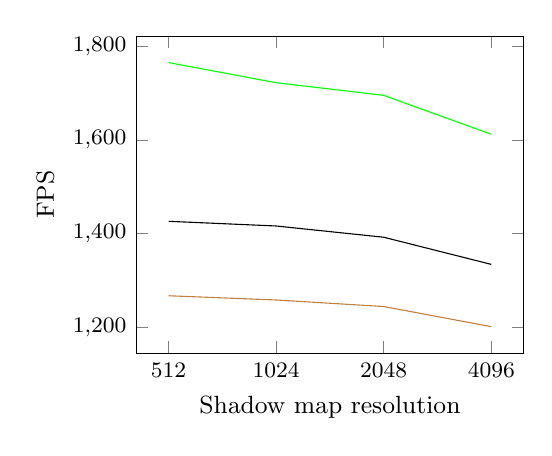
\begin{tikzpicture}
            \begin{semilogxaxis}[
                small,
                xlabel={Shadow map resolution},
                ylabel={FPS},
                xtick={512,1024,2048,4096},
                xticklabels={512,1024,2048,4096},
                % legend style={
                %     overlay,
                %     at={(1.25,0.5)},
                %     anchor=center},
                y tick label style={
                    /pgf/number format/.cd,
                        fixed,   % po zakomentowaniu os rzednych jest indeksowana wykladniczo
                        fixed, % 1.0 zamiast 1
                        precision=1,
                    /tikz/.cd
                },
                x tick label style={
                    /pgf/number format/.cd,
                        fixed,
                        fixed,
                        precision=2,
                    /tikz/.cd
                }
                ]
                \addplot [color=green]
                coordinates {
                    (512,1765)(1024,1722)(2048,1695)(4096,1612)}; %\addlegendentry{720p}
                \addplot [color=black]
                coordinates {
                    (512,1426)(1024,1416)(2048,1392)(4096,1334)}; %\addlegendentry{1080p}
                \addplot [color=brown]
                coordinates {
                    (512,1267)(1024,1258)(2048,1244)(4096,1201)}; %\addlegendentry{2k}
            \end{semilogxaxis} 
        \end{tikzpicture}
        \caption{Results for Chinese Dragon scene.}
        \label{fig:plot:bilinear_dragon}
    \end{subfigure}
    \hfill
    \begin{subfigure}[t]{0.48\textwidth}
        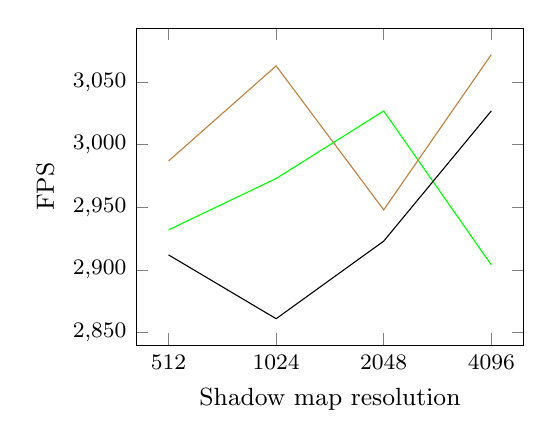
\begin{tikzpicture}
            \begin{semilogxaxis}[
                small,
                xlabel={Shadow map resolution},
                ylabel={FPS},
                xtick={512,1024,2048,4096},
                xticklabels={512,1024,2048,4096},
                % legend style={
                %     overlay,
                %     at={(1.25,0.5)},
                %     anchor=center},
                y tick label style={
                    /pgf/number format/.cd,
                        fixed,   % po zakomentowaniu os rzednych jest indeksowana wykladniczo
                        fixed, % 1.0 zamiast 1
                        precision=1,
                    /tikz/.cd
                },
                x tick label style={
                    /pgf/number format/.cd,
                        fixed,
                        fixed,
                        precision=2,
                    /tikz/.cd
                }
                ]
                \addplot [color=green]
                coordinates {
                    (512,2932)(1024,2973)(2048,3027)(4096,2904)}; %\addlegendentry{720p}
                \addplot [color=black]
                coordinates {
                    (512,2912)(1024,2861)(2048,2923)(4096,3027)}; %\addlegendentry{1080p}
                \addplot [color=brown]
                coordinates {
                    (512,2987)(1024,3063)(2048,2948)(4096,3072)}; %\addlegendentry{2k}
            \end{semilogxaxis} 
        \end{tikzpicture}
        \caption{Results for the Cube scene.}
        \label{fig:plot:bilinear_cube}
    \end{subfigure}
    
    \vspace{20pt}
    \begin{subfigure}[t]{0.48\textwidth}
        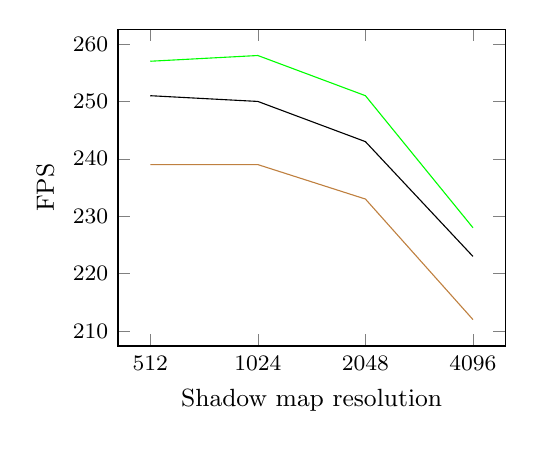
\begin{tikzpicture}
            \begin{semilogxaxis}[
                small,
                xlabel={Shadow map resolution},
                ylabel={FPS},
                xtick={512,1024,2048,4096},
                xticklabels={512,1024,2048,4096},
                % legend style={
                %     overlay,
                %     at={(1.25,0.5)},
                %     anchor=center},
                y tick label style={
                    /pgf/number format/.cd,
                        fixed,   % po zakomentowaniu os rzednych jest indeksowana wykladniczo
                        fixed, % 1.0 zamiast 1
                        precision=1,
                    /tikz/.cd
                },
                x tick label style={
                    /pgf/number format/.cd,
                        fixed,
                        fixed,
                        precision=2,
                    /tikz/.cd
                }
                ]
                \addplot [color=green]
                coordinates {
                    (512,257)(1024,258)(2048,251)(4096,228)}; %\addlegendentry{720p}
                \addplot [color=black]
                coordinates {
                    (512,251)(1024,250)(2048,243)(4096,223)}; %\addlegendentry{1080p}
                \addplot [color=brown]
                coordinates {
                    (512,239)(1024,239)(2048,233)(4096,212)}; %\addlegendentry{2k}
            \end{semilogxaxis} 
        \end{tikzpicture}
        \caption{Results for the Power Plant scene.}
        \label{fig:plot:bilinear_power}
    \end{subfigure}
    \hfill
    \begin{subfigure}[t]{0.48\textwidth}
        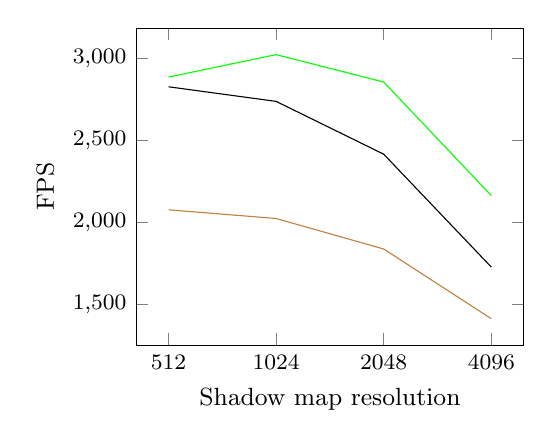
\begin{tikzpicture}
            \begin{semilogxaxis}[
                small,
                xlabel={Shadow map resolution},
                ylabel={FPS},
                xtick={512,1024,2048,4096},
                xticklabels={512,1024,2048,4096},
                % legend style={
                %     overlay,
                %     at={(1.25,0.5)},
                %     anchor=center},
                y tick label style={
                    /pgf/number format/.cd,
                        fixed,   % po zakomentowaniu os rzednych jest indeksowana wykladniczo
                        fixed, % 1.0 zamiast 1
                        precision=1,
                    /tikz/.cd
                },
                x tick label style={
                    /pgf/number format/.cd,
                        fixed,
                        fixed,
                        precision=2,
                    /tikz/.cd
                }
                ]
                \addplot [color=green]
                coordinates {
                    (512,2884)(1024,3021)(2048,2854)(4096,2162)}; %\addlegendentry{720p} here at 4k drpos <10 fps visible
                \addplot [color=black]
                coordinates {
                    (512,2825)(1024,2736)(2048,2414)(4096,1726)}; %at 4k shadow map, visible difference of few fps, sometimes... %\addlegendentry{1080p}
                \addplot [color=brown]
                coordinates {
                    (512,2075)(1024,2022)(2048,1836)(4096,1411)}; %\addlegendentry{2k}
            \end{semilogxaxis} 
        \end{tikzpicture}
        \caption{Results for the Crytek Sponza scene.}
        \label{fig:plot:bilinear_sponza}
    \end{subfigure}
    \caption{Frames per second for all test scenes, for different sizes of the shadow map and output resolutions. In green \(1280\times 720\), in black \(1920\times 1080\) and in brown \(2560\times 1440\). Rendering with the basic shadow mapping technique with bilinear filtering enabled.}
    \label{fig:plot:bilinear_results}
\end{figure}

The results are very similar, with no immediately visible drop in performance. Taking the Power Plant scene as an example, the FPS range measured at Full HD output resolution is \([251:223]\). In the shadow mapping without filtering test the FPS range was \([250:223]\). The results are the same when accounting for instabilities caused by other software and dynamic clock rates. This is interesting when compared to results of Crytek Sponza tests, where the Full HD range was \([2825:1726]\) with bilinear filtering and  \([2912:1750]\) without. Here, a significant drop in performance can be seen when using bilinear filtering. This might be caused by the fact FPS measurements are more sensitive in higher rages, as 1 FPS difference at 250 FPS is equal to 0.016ms, while 1 FPS difference at 2800 FPS is equal to only 0,000127ms. This is somewhat visible in the Crytek Sponza FPS ranges, as the upper ends have a higher difference between them than lower ends. Additionally, since the Power Plant is a much heavier scene performance-wise, the GPU has much more work to perform and the slowdown from using bilinear filtering can get masked better. When toggling bilinear filtering on and off during testing, the FPS readout would most of the time stay stable within reasonable FPS ranges. It seems that the cost of hardware bilinear filtering is indeed insignificant in realistic scenarios, where the GPU is fully utilized.

The effect on the final rendered result is on the other hand very significant, especially at lower shadow map resolutions, as presented in figure \ref{fig:test_bilinear_dragon_screens}. The shadow boundaries get smoother, which improves the visuals even at low shadow map resolutions. The texels are less noticeable and the shape is more easily readable as a shadow.

\begin{figure}[h]
    \centering
    \begin{subfigure}[t]{0.48\textwidth}
		\centering
        \includegraphics[width=\textwidth]{./graf/tests/basic/cropped/dragon_basic_fhd_512.png}
        \caption{The Chinese Dragon rendered with a \(512\times 512\) shadow map with no filtering.}
    \end{subfigure}
	\hfill
    \begin{subfigure}[t]{0.48\textwidth}
		\centering
        \includegraphics[width=\textwidth]{./graf/tests/bilinear/cropped/dragon_bilinear_fhd_512.png}
        \caption{The Chinese Dragon rendered with a \(512\times 512\) shadow map with bilinear filtering.}
    \end{subfigure}
    \begin{subfigure}[t]{0.48\textwidth}
		\centering
        \includegraphics[width=\textwidth]{./graf/tests/basic/cropped/dragon_basic_fhd_4096.png}
        \caption{The Chinese Dragon rendered with a \(4096\times 4096\) shadow map with no filtering.}
    \end{subfigure}
	\hfill
    \begin{subfigure}[t]{0.48\textwidth}
		\centering
        \includegraphics[width=\textwidth]{./graf/tests/bilinear/cropped/dragon_bilinear_fhd_4096.png}
        \caption{The Chinese Dragon rendered with a \(4096\times 4096\) shadow map with bilinear filtering.}
    \end{subfigure}

    \caption{The Chinese Dragon rendered with and without bilinear comparison filtering.}
    \label{fig:test_bilinear_dragon_screens}
\end{figure}

Unfortunately, this filtering means that biasing has to be adjusted, as samples will be taken around the original position. This results in visible shadow acne, especially at lower shadow map resolutions, where shadow map texels cover a larger area on screen. It's noteworthy that, while there will be more pixels that erroneously self-shadow, the contrast of such artifacts will be smaller. This can help hide them at higher shadow map resolutions.

\subsubsection{Percentage-closer filtering}
PCF is another filtering technique that allows for the creation of arbitrarily sized filter kernels used to filter the results of shadow computations. For the performance tests, the shadow map resolution will be kept constant to measure how kernel size and output resolution affect the FPS counts. Shadow map resolution does not impact the results in the context of this technique, apart from the performance degradation with higher shadow map resolutions observed in previous tests. The results for all scenes, for different square filter kernel sizes and output resolutions are presented in Fig. \ref{fig:plot:pcf_results}.
\begin{figure}[h]
    \centering
    \begin{subfigure}[t]{0.48\textwidth}
        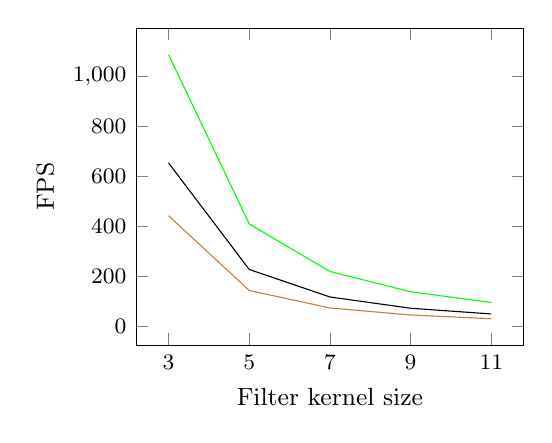
\begin{tikzpicture}
            \begin{axis}[
                small,
                xlabel={Filter kernel size},
                ylabel={FPS},
                xtick={3,5,7,9,11},
                xticklabels={3,5,7,9,11},
                % legend style={
                %     overlay,
                %     at={(1.25,0.5)},
                %     anchor=center},
                y tick label style={
                    /pgf/number format/.cd,
                        fixed,   % po zakomentowaniu os rzednych jest indeksowana wykladniczo
                        fixed, % 1.0 zamiast 1
                        precision=1,
                    /tikz/.cd
                },
                x tick label style={
                    /pgf/number format/.cd,
                        fixed,
                        fixed,
                        precision=2,
                    /tikz/.cd
                }
                ]
                \addplot [color=green]
                coordinates {
                    (3,1087)(5,410)(7,220)(9,139)(11,96)}; %\addlegendentry{720p}
                \addplot [color=black]
                coordinates {
                    (3,654)(5,228)(7,118)(9,73)(11,50)}; %\addlegendentry{1080p}
                \addplot [color=brown]
                coordinates {
                    (3,443)(5,144)(7,74)(9,46)(11,31)}; %\addlegendentry{2k}
            \end{axis} 
        \end{tikzpicture}
        \caption{Results for Chinese Dragon scene.}
        \label{fig:plot:pcf_dragon}
    \end{subfigure}
    \hfill
    \begin{subfigure}[t]{0.48\textwidth}
        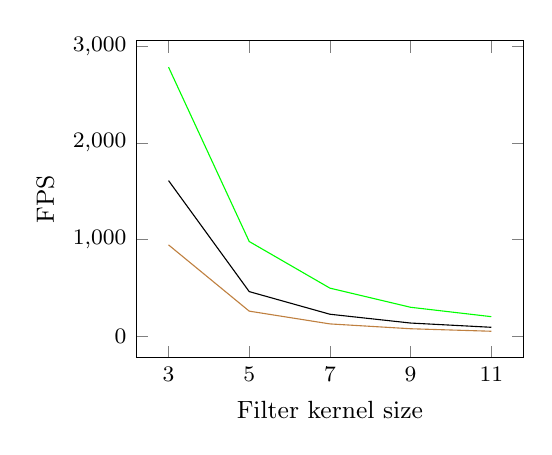
\begin{tikzpicture}
            \begin{axis}[
                small,
                xlabel={Filter kernel size},
                ylabel={FPS},
                xtick={3,5,7,9,11},
                xticklabels={3,5,7,9,11},
                % legend style={
                %     overlay,
                %     at={(1.25,0.5)},
                %     anchor=center},
                y tick label style={
                    /pgf/number format/.cd,
                        fixed,   % po zakomentowaniu os rzednych jest indeksowana wykladniczo
                        fixed, % 1.0 zamiast 1
                        precision=1,
                    /tikz/.cd
                },
                x tick label style={
                    /pgf/number format/.cd,
                        fixed,
                        fixed,
                        precision=2,
                    /tikz/.cd
                }
                ]
                \addplot [color=green]
                coordinates {
                    (3,2783)(5,980)(7,498)(9,300)(11,203)}; %\addlegendentry{720p}
                \addplot [color=black]
                coordinates {
                    (3,1610)(5,462)(7,228)(9,137)(11,93)}; %\addlegendentry{1080p}
                \addplot [color=brown]
                coordinates {
                    (3,945)(5,260)(7,128)(9,78)(11,52)}; %\addlegendentry{2k}
            \end{axis} 
        \end{tikzpicture}
        \caption{Results for the Cube scene.}
        \label{fig:plot:pcf_cube}
    \end{subfigure}

    \vspace{20pt}
    \begin{subfigure}[t]{0.48\textwidth}
        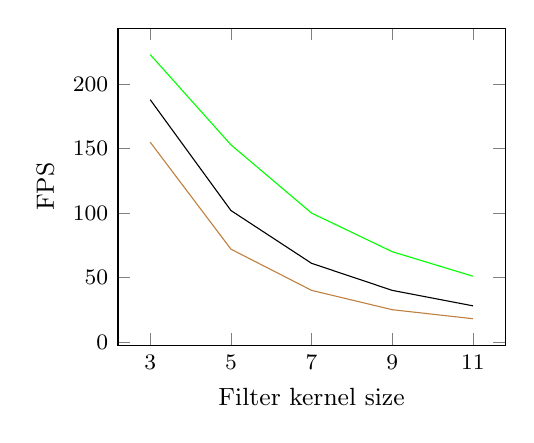
\begin{tikzpicture}
            \begin{axis}[
                small,
                xlabel={Filter kernel size},
                ylabel={FPS},
                xtick={3,5,7,9,11},
                xticklabels={3,5,7,9,11},
                % legend style={
                %     overlay,
                %     at={(1.25,0.5)},
                %     anchor=center},
                y tick label style={
                    /pgf/number format/.cd,
                        fixed,   % po zakomentowaniu os rzednych jest indeksowana wykladniczo
                        fixed, % 1.0 zamiast 1
                        precision=1,
                    /tikz/.cd
                },
                x tick label style={
                    /pgf/number format/.cd,
                        fixed,
                        fixed,
                        precision=2,
                    /tikz/.cd
                }
                ]
                \addplot [color=green]
                coordinates {
                    (3,223)(5,153)(7,100)(9,70)(11,51)}; %\addlegendentry{720p}
                \addplot [color=black]
                coordinates {
                    (3,188)(5,102)(7,61)(9,40)(11,28)}; %\addlegendentry{1080p}
                \addplot [color=brown]
                coordinates {
                    (3,155)(5,72)(7,40)(9,25)(11,18)}; %\addlegendentry{2k}
            \end{axis} 
        \end{tikzpicture}
        \caption{Results for the Power Plant scene.}
        \label{fig:plot:pcf_power}
    \end{subfigure}
    \hfill
    \begin{subfigure}[t]{0.48\textwidth}
        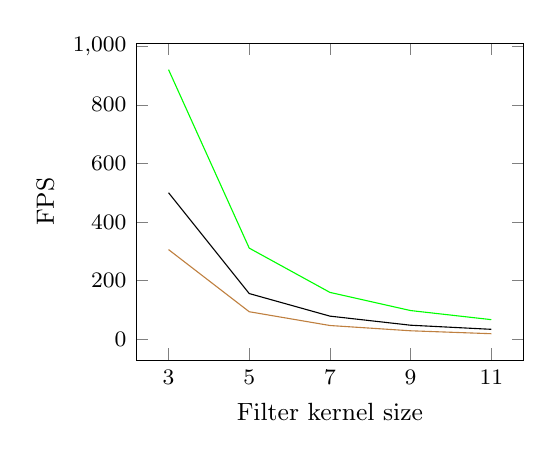
\begin{tikzpicture}
            \begin{axis}[
                small,
                xlabel={Filter kernel size},
                ylabel={FPS},
                xtick={3,5,7,9,11},
                xticklabels={3,5,7,9,11},
                % legend style={
                %     overlay,
                %     at={(1.25,0.5)},
                %     anchor=center},
                y tick label style={
                    /pgf/number format/.cd,
                        fixed,   % po zakomentowaniu os rzednych jest indeksowana wykladniczo
                        fixed, % 1.0 zamiast 1
                        precision=1,
                    /tikz/.cd
                },
                x tick label style={
                    /pgf/number format/.cd,
                        fixed,
                        fixed,
                        precision=2,
                    /tikz/.cd
                }
                ]
                \addplot [color=green]
                coordinates {
                    (3,920)(5,311)(7,160)(9,98)(11,67)}; %\addlegendentry{720p}
                \addplot [color=black]
                coordinates {
                    (3,500)(5,156)(7,79)(9,48)(11,34)}; %\addlegendentry{1080p}
                \addplot [color=brown]
                coordinates {
                    (3,306)(5,94)(7,47)(9,29)(11,19)}; %\addlegendentry{2k}
            \end{axis} 
        \end{tikzpicture}
        \caption{Results for the Crytek Sponza scene.}
        \label{fig:plot:pcf_sponza}
    \end{subfigure}
    \caption{Frames per second for all test scenes, for different sizes of the filter kernel and output resolutions. In green \(1280\times 720\), in black \(1920\times 1080\) and in brown \(2560\times 1440\). Rendering with the basic shadow mapping technique with PCF at constant shadow map size \(1024\times 1024\).}
    \label{fig:plot:pcf_results}
\end{figure}

The results show performance dropping exponentially with regard to increasing filter kernel size. This is expected, as for a kernel of size \(n\) there are \(n^2\) depth comparisons performed. This fact makes high kernel sizes impractical and limits the usability of the approach. A larger smoothing effect is better achieved by using a scale factor to scale the sample offsets within the filter kernel than by increasing the kernel size.

\begin{figure}[p]
    \centering
    \begin{subfigure}[t]{0.48\textwidth}
		\centering
        \includegraphics[width=\textwidth]{./graf/tests/pcf/cropped/dragon_pcf_fhd_1024_3x3.png}
        \caption{The shadow of the Chinese Dragon filtered with a \(3\times 3\) kernel.}
    \end{subfigure}
	\hfill
    \begin{subfigure}[t]{0.48\textwidth}
		\centering
        \includegraphics[width=\textwidth]{./graf/tests/pcf/cropped/dragon_pcf_fhd_1024_11x11.png}
        \caption{The shadow of the Chinese Dragon filtered with an \(11\times 11\) kernel.}
    \end{subfigure}

    \begin{subfigure}[t]{0.48\textwidth}
		\centering
        \includegraphics[width=\textwidth]{./graf/tests/pcf/cropped/dragon_pcf_fhd_1024_3x3_offset05.png}
        \caption{The shadow of the Chinese Dragon filtered with a \(3\times 3\) kernel and a scale of \(0.5\) applied to each kernel offset.}
    \end{subfigure}
    \hfill
    \begin{subfigure}[t]{0.48\textwidth}
		\centering
        \includegraphics[width=\textwidth]{./graf/tests/pcf/cropped/dragon_pcf_fhd_1024_11x11_offset05.png}
        \caption{The shadow of the Chinese Dragon filtered with an \(11\times 11\) kernel and a scale of \(0.5\) applied to each kernel offset.}
    \end{subfigure}

    \begin{subfigure}[t]{0.48\textwidth}
		\centering
        \includegraphics[width=\textwidth]{./graf/tests/pcf/cropped/dragon_pcf_fhd_1024_3x3_offset3.png}
        \caption{The shadow of the Chinese Dragon filtered with a \(3\times 3\) kernel and a scale of \(3\) applied to each kernel offset.}
    \end{subfigure}
	\hfill
    \begin{subfigure}[t]{0.48\textwidth}
		\centering
        \includegraphics[width=\textwidth]{./graf/tests/pcf/cropped/dragon_pcf_fhd_1024_11x11_offset3.png}
        \caption{The shadow of the Chinese Dragon filtered with an \(11\times 11\) kernel and a scale of \(3\) applied to each kernel offset.}
    \end{subfigure}    

    \caption{The Chinese Dragon rendered with \(3\times 3\) and \(11\times 11\) kernels with different offset scales.}
    \label{fig:test_pcf_dragon_screens}
\end{figure}

During testing interesting behavior was observed. In all tests, when the application was running with its initial kernel parameter unchanged, the frame rate would be much higher than at the same kernel size after any change to it was made. This difference in some cases was as large as the entire FPS value after a change, meaning the loss of half the frame rate. The reason for this is not known, because default initialization and optimization of the code path is unlikely, as neither the shader code nor the compiler know of the initial settings that will be used for the kernel size. All results shown in Fig. \ref{fig:plot:pcf_results} present FPS values after the initial change was made.

The appearance of shadows rendered with different sizes of kernels and offsets is presented in Fig. \ref{fig:test_pcf_dragon_screens}.
Banding is very much visible in the smoothed areas of the shadows, even with the largest kernel. This is because of the limited range of shades that can be produced in these transitional areas. A transition that appears smoother can be achieved by setting a smaller than 1 offset scale, but that limits the size of the smoothed shadow areas. Additionally, texel boundaries are always visible with this method.

The usage of even the smallest \(3\times 3\) kernel requires adjusting the depth bias to get clean results. The larger the kernel, the more bias is needed. This could be partially alleviated by using the distance from the kernel center to scale a bias that is added before the comparison happens, but overall bias would still depend on receiver orientations and would need to be adjusted per-scene.

\begin{figure}[h]
    \centering
    \begin{subfigure}[t]{0.45\textwidth}
		\centering
        \includegraphics[width=\textwidth]{./graf/tests/pcf/cropped/dragon_pcf_fhd_512_3x3.png}
        \caption{The Chinese Dragon rendered with basic \(3\times 3\) PCF.}
    \end{subfigure}
	\hfill
    \begin{subfigure}[t]{0.45\textwidth}
		\centering
        \includegraphics[width=\textwidth]{./graf/tests/pcf/cropped/dragon_pcf_fhd_512_3x3_bilinear.png}
        \caption{The Chinese Dragon rendered with \(3\times 3\) PCF enhanced by bilinear filtering.}
    \end{subfigure}
    \begin{subfigure}[t]{0.45\textwidth}
		\centering
        \includegraphics[width=\textwidth]{./graf/tests/pcf/cropped/dragon_pcf_fhd_512_11x11.png}
        \caption{The Chinese Dragon rendered with basic \(11\times 11\) PCF.}
    \end{subfigure}
	\hfill
    \begin{subfigure}[t]{0.45\textwidth}
		\centering
        \includegraphics[width=\textwidth]{./graf/tests/pcf/cropped/dragon_pcf_fhd_512_11x11_bilinear.png}
        \caption{The Chinese Dragon rendered with \(11\times 11\) PCF enhanced by bilinear filtering.}
    \end{subfigure}

    \caption{The Chinese Dragon rendered with PCF and with and without additional bilinear comparison filtering, using a \(512\times 512\) shadow map resolution.}
    \label{fig:test_pfc_bilinear_dragon_screens}
\end{figure}

The performance cost and underwhelming results make this technique mainly a stepping stone for more robust approaches. It is not practical to use it in real applications that need to run in real time. There is however one adjustment that can be made to significantly improve the shadow's appearance produced by PCF. As established in section \ref{section:test_bilinear}, hardware bilinear comparison filtering comes at virtually no performance cost. It can be applied to PCF, the results of which are shown in Fig. \ref{fig:test_pfc_bilinear_dragon_screens}

These results show that bilinear comparison filtering combined with PCF can lead to a great improvement of the visuals, even at kernel sizes as small as \(3\times 3\). Additionally, the shadow map used there has only \(512\times 512\) resolution, making it a very performant option. The impractical kernel size \(11\times 11\), when combined with bilinear filtering gives very smooth results, without any banding, hiding the texel boundaries very well, especially considering the low resolution of the shadow map.

\subsubsection{Adaptive percentage-closer filtering}

\subsection{Soft shadows with shadow maps}

\subsubsection{PCSS}

% \begin{table}
% \centering
% \caption{A caption of a table is ABOVE it.}
% \label{id:tab:wyniki}
% \begin{tabular}{rrrrrrrr}
% \toprule
% 	         &                                     \multicolumn{7}{c}{method}                                      \\
% 	         \cmidrule{2-8}
% 	         &         &         &        \multicolumn{3}{c}{alg. 3}        & \multicolumn{2}{c}{alg. 4, $\gamma = 2$} \\
% 	         \cmidrule(r){4-6}\cmidrule(r){7-8}
% 	$\zeta$ &     alg. 1 &   alg. 2 & $\alpha= 1.5$ & $\alpha= 2$ & $\alpha= 3$ &   $\beta = 0.1$  &   $\beta = -0.1$ \\
% \midrule
% 	       0 &  8.3250 & 1.45305 &       7.5791 &    14.8517 &    20.0028 & 1.16396 &                       1.1365 \\
% 	       5 &  0.6111 & 2.27126 &       6.9952 &    13.8560 &    18.6064 & 1.18659 &                       1.1630 \\
% 	      10 & 11.6126 & 2.69218 &       6.2520 &    12.5202 &    16.8278 & 1.23180 &                       1.2045 \\
% 	      15 &  0.5665 & 2.95046 &       5.7753 &    11.4588 &    15.4837 & 1.25131 &                       1.2614 \\
% 	      20 & 15.8728 & 3.07225 &       5.3071 &    10.3935 &    13.8738 & 1.25307 &                       1.2217 \\
% 	      25 &  0.9791 & 3.19034 &       5.4575 &     9.9533 &    13.0721 & 1.27104 &                       1.2640 \\
% 	      30 &  2.0228 & 3.27474 &       5.7461 &     9.7164 &    12.2637 & 1.33404 &                       1.3209 \\
% 	      35 & 13.4210 & 3.36086 &       6.6735 &    10.0442 &    12.0270 & 1.35385 &                       1.3059 \\
% 	      40 & 13.2226 & 3.36420 &       7.7248 &    10.4495 &    12.0379 & 1.34919 &                       1.2768 \\
% 	      45 & 12.8445 & 3.47436 &       8.5539 &    10.8552 &    12.2773 & 1.42303 &                       1.4362 \\
% 	      50 & 12.9245 & 3.58228 &       9.2702 &    11.2183 &    12.3990 & 1.40922 &                       1.3724 \\
% \bottomrule
% \end{tabular}
% \end{table}  

% The table is here too \ref{id:tab:wyniki}

%%%%%%%%%%%%%%%%%%%%%
% FIGURE FROM FILE
%
% \begin{figure}
% \centering
% \includegraphics[width=0.5\textwidth]{./graf/politechnika_sl_logo_bw_pion_en.pdf}
% \caption{Caption of a figure is always below the figure.}
% \label{fig:label}
% \end{figure}

% Fig. \ref{fig:label} presents asdasd

% \begin{figure}
% \includegraphics[width=0.5\textwidth]{./graf/test_image.jpg}
% \caption{Caption of a figure is always below the figure akakak.}
% \label{fig:duped_image3}
% \end{figure}

% some citation of the above \ref{fig:duped_image3}

%%%%%%%%%%%%%%%%%%%%%
%
%%%%%%%%%%%%%%%%%%%%
%% SUBFIGURES
%
% \begin{figure}
% \centering
% \begin{subfigure}{0.4\textwidth}
%    \includegraphics[width=\textwidth]{./graf/politechnika_sl_logo_bw_pion_en.pdf}
%    \caption{Upper left figure.}
%    \label{fig:upper-left}
% \end{subfigure}
% \hfill
% \begin{subfigure}{0.4\textwidth}
%    \includegraphics[width=\textwidth]{./graf/politechnika_sl_logo_bw_pion_en.pdf}
%    \caption{Upper right figure.}
%    \label{fig:upper-right}
% \end{subfigure}

% \begin{subfigure}{0.4\textwidth}
%    \includegraphics[width=\textwidth]{./graf/politechnika_sl_logo_bw_pion_en.pdf}
%    \caption{Lower left figure.}
%    \label{fig:lower-left}
% \end{subfigure}
% \hfill
% \begin{subfigure}{0.4\textwidth}
%    \includegraphics[width=\textwidth]{./graf/politechnika_sl_logo_bw_pion_en.pdf}
%    \caption{Lower right figure.}
%    \label{fig:lower-right}
% \end{subfigure}
       
% \caption{Common caption for all subfigures.}
% \label{fig:subfigures}
% \end{figure}
% Fig. \ref{fig:subfigures} presents very important information, eg. Fig. \ref{fig:upper-right} is an upper right subfigure.
%%%%%%%%%%%%%%%%%%%%%



% \begin{figure}
% \centering
% \begin{tikzpicture}
% \begin{axis}[
%    y tick label style={
%        /pgf/number format/.cd,
%            fixed,   % po zakomentowaniu os rzednych jest indeksowana wykladniczo
%            fixed zerofill, % 1.0 zamiast 1
%            precision=1,
%        /tikz/.cd
%    },
%    x tick label style={
%        /pgf/number format/.cd,
%            fixed,
%            fixed zerofill,
%            precision=2,
%        /tikz/.cd
%    }
% ]
% \addplot [domain=0.0:0.1] {rnd};
% \end{axis} 
% \end{tikzpicture}
% \caption{Figure caption is BELOW the figure.}
% \label{fig:3}
% \end{figure}

% \begin{figure}
% \centering
% \includegraphics[width=0.5\textwidth]{./graf/politechnika_sl_logo_bw_pion_en.pdf}
% \caption{Caption of a figure is always below the figure akakak.}
% \label{fig:3}
% \end{figure}

% some citation of the above \ref{fig:3}

% \begin{figure}
% \begin{lstlisting}
% if (_nClusters < 1)
% 	throw std::string ("unknown number of clusters");
% if (_nIterations < 1 and _epsilon < 0)
% 	throw std::string ("You should set a maximal number of iteration or minimal difference -- epsilon.");
% if (_nIterations > 0 and _epsilon > 0)
% 	throw std::string ("Both number of iterations and minimal epsilon set -- you should set either number of iterations or minimal epsilon.");
% \end{lstlisting}
% \caption{Example of pseudocode.}
% \end{figure}

\chapter{Summary}
\label{section:chapter_5}

% \begin{itemize}
% \item What problem have I solved?
% \item How have I solved the problem?
% \item What are pros and cons of my solutions?
% \item Can I state some recommendations?
% \end{itemize}

% \begin{itemize}
% \item synthetic description of performed work
% \item conclusions
% \item  future development, potential future research
% \item Has the objective been reached?
% \end{itemize}

Within the realm of computer graphics rendering, many approaches to render various physical phenomena exist. Shadow rendering is no exception, offering a plethora of choices varying in visual robustness, achievable performance and realism. This thesis analyzed some of the techniques meant for real-time shadow rendering, providing their background and explaining their algorithms. Within the scope of the thesis, a test application was built in \textit{C++} using the \textit{DirectX 12} graphics API. The application implemented chosen techniques and allowed them to be tested and compared against each other on the basis of performance and visual quality.

The tests demonstrated that each technique has its pros and cons. The best  quality of the rendered results in percentage-closer soft shadows is reflected in the heavy performance requirements. Fast basic shadow mapping would look out of place within a modern renderer, giving unrealistic hard shadows and heavy aliasing. A solid middle ground seems to be variance shadow mapping, which is exceptionally performant and can eliminate aliasing entirely. Adaptive percentage-closer filtering produces pleasant results and attempts to improve the performance of basic PCF with a clever branching algorithm. Albeit offering worse performance than VSM, it can retain more detail in the shadows and does not suffer from light bleeding.

Within the scope of this thesis six approaches to shadow rendering were implemented and tested. In the future it would be worthwhile to investigate more advanced and modern rendering techniques to see how some problems present in the ones already covered are getting solved and in what directions the field is heading.

\backmatter

% \bibliographystyle{plain}  % bibtex
% \bibliography{biblio/biblio.bib} % bibtex
\printbibliography           % biblatex
\addcontentsline{toc}{chapter}{Bibliography}

\begin{appendices}

\chapter{Technical documentation}

\section{Building the test application}
The test application uses \textit{CMake} to get all the dependencies and create a buildable \textit{MSVC} project. The application was built using \textit{Visual Studio Code} and \textit{CMake Tools} extension. In the \textit{CMake Tools} extension tab the configuration, for example `msvc Release', should be selected. After that the build target `ShadowRendering' and a preset have to be set. The extension will then begin fetching the dependencies and configuring the project. Once ready the program can be built. The only dependency that is not handled by \textit{CMake} is the \textit{Windows SDK}. The user has to install it manually in the default installation location. The executable is built into an appropriate location in the /build directory, depending on the configuration.

\section{Using the test application}
Once launched, the application will load the \textit{Cube} scene and present a window containing the rendered output. \textit{ImGUI} can be toggled with the `H' key. It contains information on controls, allows selection of rendering modes and provides brief explanations. It also displays the FPS and frame time of the application if the widget is enabled.

\section{Profiling the test application}
To profile the test application, an executable of \textit{TracyProfiler} can be downloaded from its \textit{GitHub} repository. First the tracy-profiler.exe should be run, then the test application. The test application should be listed in \textit{Tracy} as ready for profiling. Upon connecting, data gathering will begin immediately and frames will start appearing in the \textit{Tracy} GUI. They can be later analyzed and inspected, for example by checking how the GPU is utilized, inspecting the time the CPU is waiting for the GPU or analyzing the timing statistics that \textit{Tracy} provides. % technical documentation (optional!)

\chapter{List of abbreviations and symbols}

\begin{itemize}
% chapter 2
\item[CGI] computer-generated imagery
\item[CAD] computer-aided design
\item[FPS] frames per second
\item[PSM] perspective shadow maps
\item[LiSPSM] light space perspective shadow maps
\item[PCF] percentage-closer filtering
\item[VSM] variance shadow maps
\item[LVSM] layered variance shadow maps
\item[PCSS] percentage-closer soft shadows
\item[MSM] moment shadow mapping
\item[RBSM] revectorization-based shadow mapping

% chapter 3
\item[NDC] normalized device coordinates
\item[WVP] world--view--projection
\item[API] application programming interface
\item[DSV] Depth Stencil View
\item[SRV] Shader resource view

% \item[$N$] cardinality of data set
% \item[$\mu$] membership function of a fuzzy set
% \item[$\mathbb{E}$] set of edges of a graph
% \item[$\mathcal{L}$] Laplace transformation
\end{itemize} % abbreviations and symbols

\chapter{List of additional files in~electronic submission}

Additional files uploaded to the system include:
\begin{itemize}
\item source code of the test application,
\item the \textit{Cube} test scene and sample texture,
\item a video file showing the running test application
\end{itemize}
 % additional files

\listoffigures
\addcontentsline{toc}{chapter}{List of figures}
\listoftables
\addcontentsline{toc}{chapter}{List of tables}

\end{appendices}

\end{document}


%% Finis coronat opus.
